\clearpage
\setcounter{page}{1}
\maketitlesupplementary
\section{Introduction}
In this supplementary material, we provide comprehensive experimental details, visual examples and extended analyses to support the findings of the main manuscript.
%
To be specific, the supplementary material is organized as follows:
%
\begin{enumerate}
\item \textbf{Detailed description of our caption generation pipeline and more examples from different datasets:}
\begin{itemize}
    \item Detailed description of the caption generation pipeline
    \item More examples from the person/vehicle ReID datasets
\end{itemize}
\item \textbf{Details of the proposed modules and experiments:}
\begin{itemize}
    \item Implementation details of the proposed modules
    \item More explanations of models in the ablation study
\end{itemize}
\item \textbf{Module validation and hyper-parameter analysis:}
\begin{itemize}
    \item Analysis of model parameters and performance
    \item Comparison with different inverse directions in IMFE
    \item Comparison with CLIP-based method
    \item Training efficiency comparison
    \item Effect of text with different modalities combination
    \item Exploration of extreme cases with missing text
    \item Effect of key modules on vehicle dataset
    \item Hyper-parameter analysis for the vehicle dataset
\end{itemize}
\item \textbf{Visualization analysis of IDEA:}
\begin{itemize}
    \item Visualization of multi-modal ranking list
    \item Visualization of the channel activation maps
\end{itemize}
\end{enumerate}
%
These analyses provide a deeper understanding of our constructed datasets, the proposed modules and experimental results, further validating the effectiveness of our method.
%
\section{Multi-modal Caption Generation}
\subsection{Details of the Caption Generation Pipeline}
To bridge the gap in multi-modal object ReID captioning, we propose a novel caption generation pipeline that leverages MLLMs to generate informative text descriptions.
%
Specifically, our pipeline consists of two steps: (1) Caption Generation and (2) Attribute Extraction.
%
Without loss of generality, we take the multi-modal person ReID dataset as an example to illustrate the caption generation pipeline.
%
\textbf{Caption Generation:}
%
The unique characteristics of multi-spectral images and the limitations of MLLMs in captioning make simultaneous annotation of paired multi-spectral images challenging.
%
When presented with images from multiple spectra, MLLMs often focus on shared semantic information while neglecting modality-specific details.
%
To address this, we design modality-specific templates to annotate each spectrum independently, ensuring rich and detailed semantic descriptions.
%
Specifically, this caption generation step offers two main advantages.
%
First, it enhances modality-specific descriptions by simplifying the captioning task, enabling the model to focus on detailed attributes unique to each spectrum.
%
Second, it broadens applicability by supporting more cases such as text-to-image ReID in the infrared spectrum, which is particularly advantageous in challenging visual environments.
%
Technically, our modality-specific templates consist of three key components: a modality-specific prefix, a generic annotation template and an anti-hallucination instruction.
\begin{enumerate}
    \item \textbf{Modality-specific Prefix:} Directs the model to focus on a particular spectrum (e.g., RGB, NIR, or TIR), providing a detailed prompt to describe key attributes such as clothing, hairstyle and belongings:
    \begin{quote}
      \small
      \textit{“Write a comprehensive description of the person's overall appearance based on the [RGB/NIR/TIR] image, strictly following this template. Include the following attributes: 'upper garment', 'lower garment', 'shoes', 'hairstyle', 'gender', 'age group' and 'belongings'. Use specific details, including color, patterns and texture details. Please follow this structure: ”}
    \end{quote}
    \item \textbf{Generic Annotation Template:} Ensures consistency across captions with the following structure:
    \begin{quote}
      \small
    \textit{“The \{Gender\} is wearing a \{Upper\_Color\} \{Upper\_Garment\} with \{Lower\_Color\} \{Lower\_Garment\} and \{Shoe\_Color\} \{Shoes\}. The \{Gender\} has \{Hairstyle\} \{Hair\_Color\} hair and appears to be \{Age\_Group\}. The \{Gender\} is carrying \{Belongings\}."}
    \end{quote}
    \item \textbf{Anti-hallucination Instruction:} Prevents imagined details~\cite{tan2024harnessing} by explicitly guiding the model to focus only on visible attributes:
    \begin{quote}
      \small
    \textit{“If certain attributes are not visible, ignore them. Do not imagine contents not present in the image. Adhere strictly to the format without adding extra explanations."}
    \end{quote}
\end{enumerate}
%
By combining images from specific spectra with their corresponding templates, MLLMs generate tailored and comprehensive text descriptions for each modality.
%
This approach provides detailed semantic information and effectively addresses the challenges of multi-modal data annotation.
%
\begin{figure*}[t]
  \centering
    \resizebox{0.92\textwidth}{!}
    {
  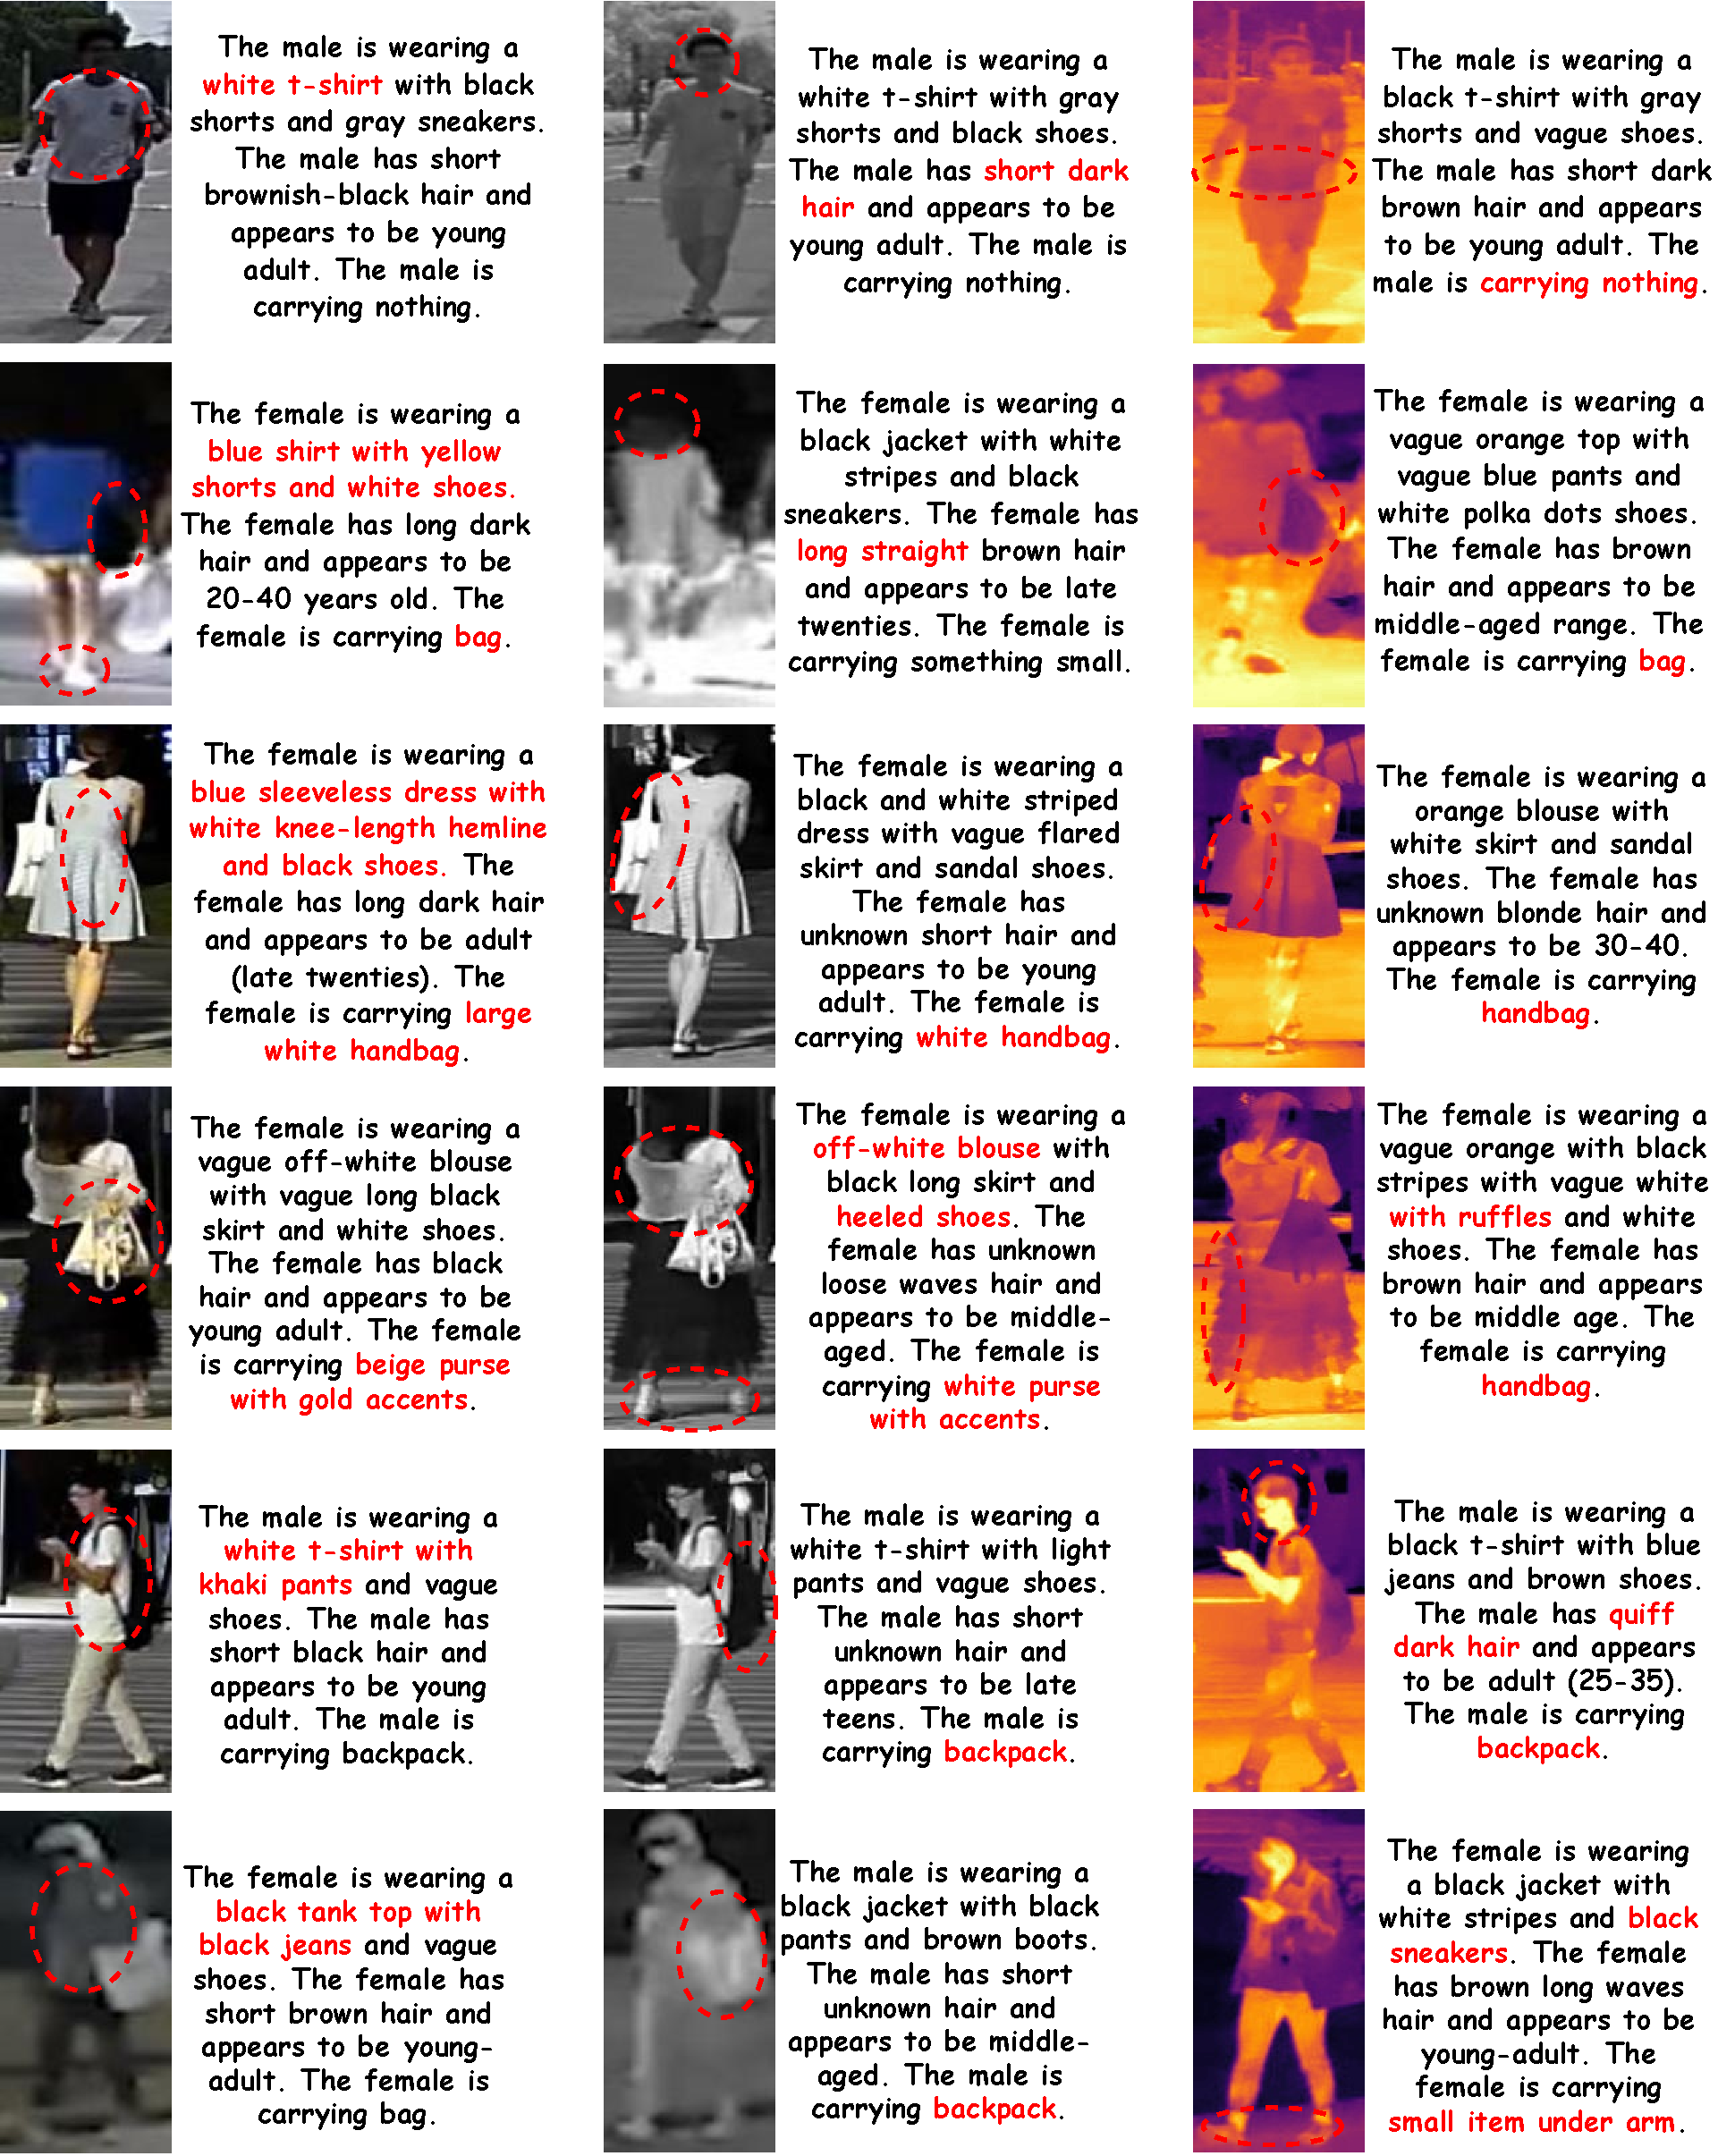
\includegraphics[width=1.\linewidth]{sec/supp_img/More_Instance_Person.pdf}
  }
  \vspace{-2mm}
   \caption{More examples from the multi-modal person ReID dataset RGBNT201.}
  \label{fig:more_instance_person}
  \vspace{-6mm}
\end{figure*}
%~~~~~~~~~~~~~~~~~~~~~~~~~~~~~~~~
\begin{figure*}[t]
  \centering
    \resizebox{0.96\textwidth}{!}
    {
  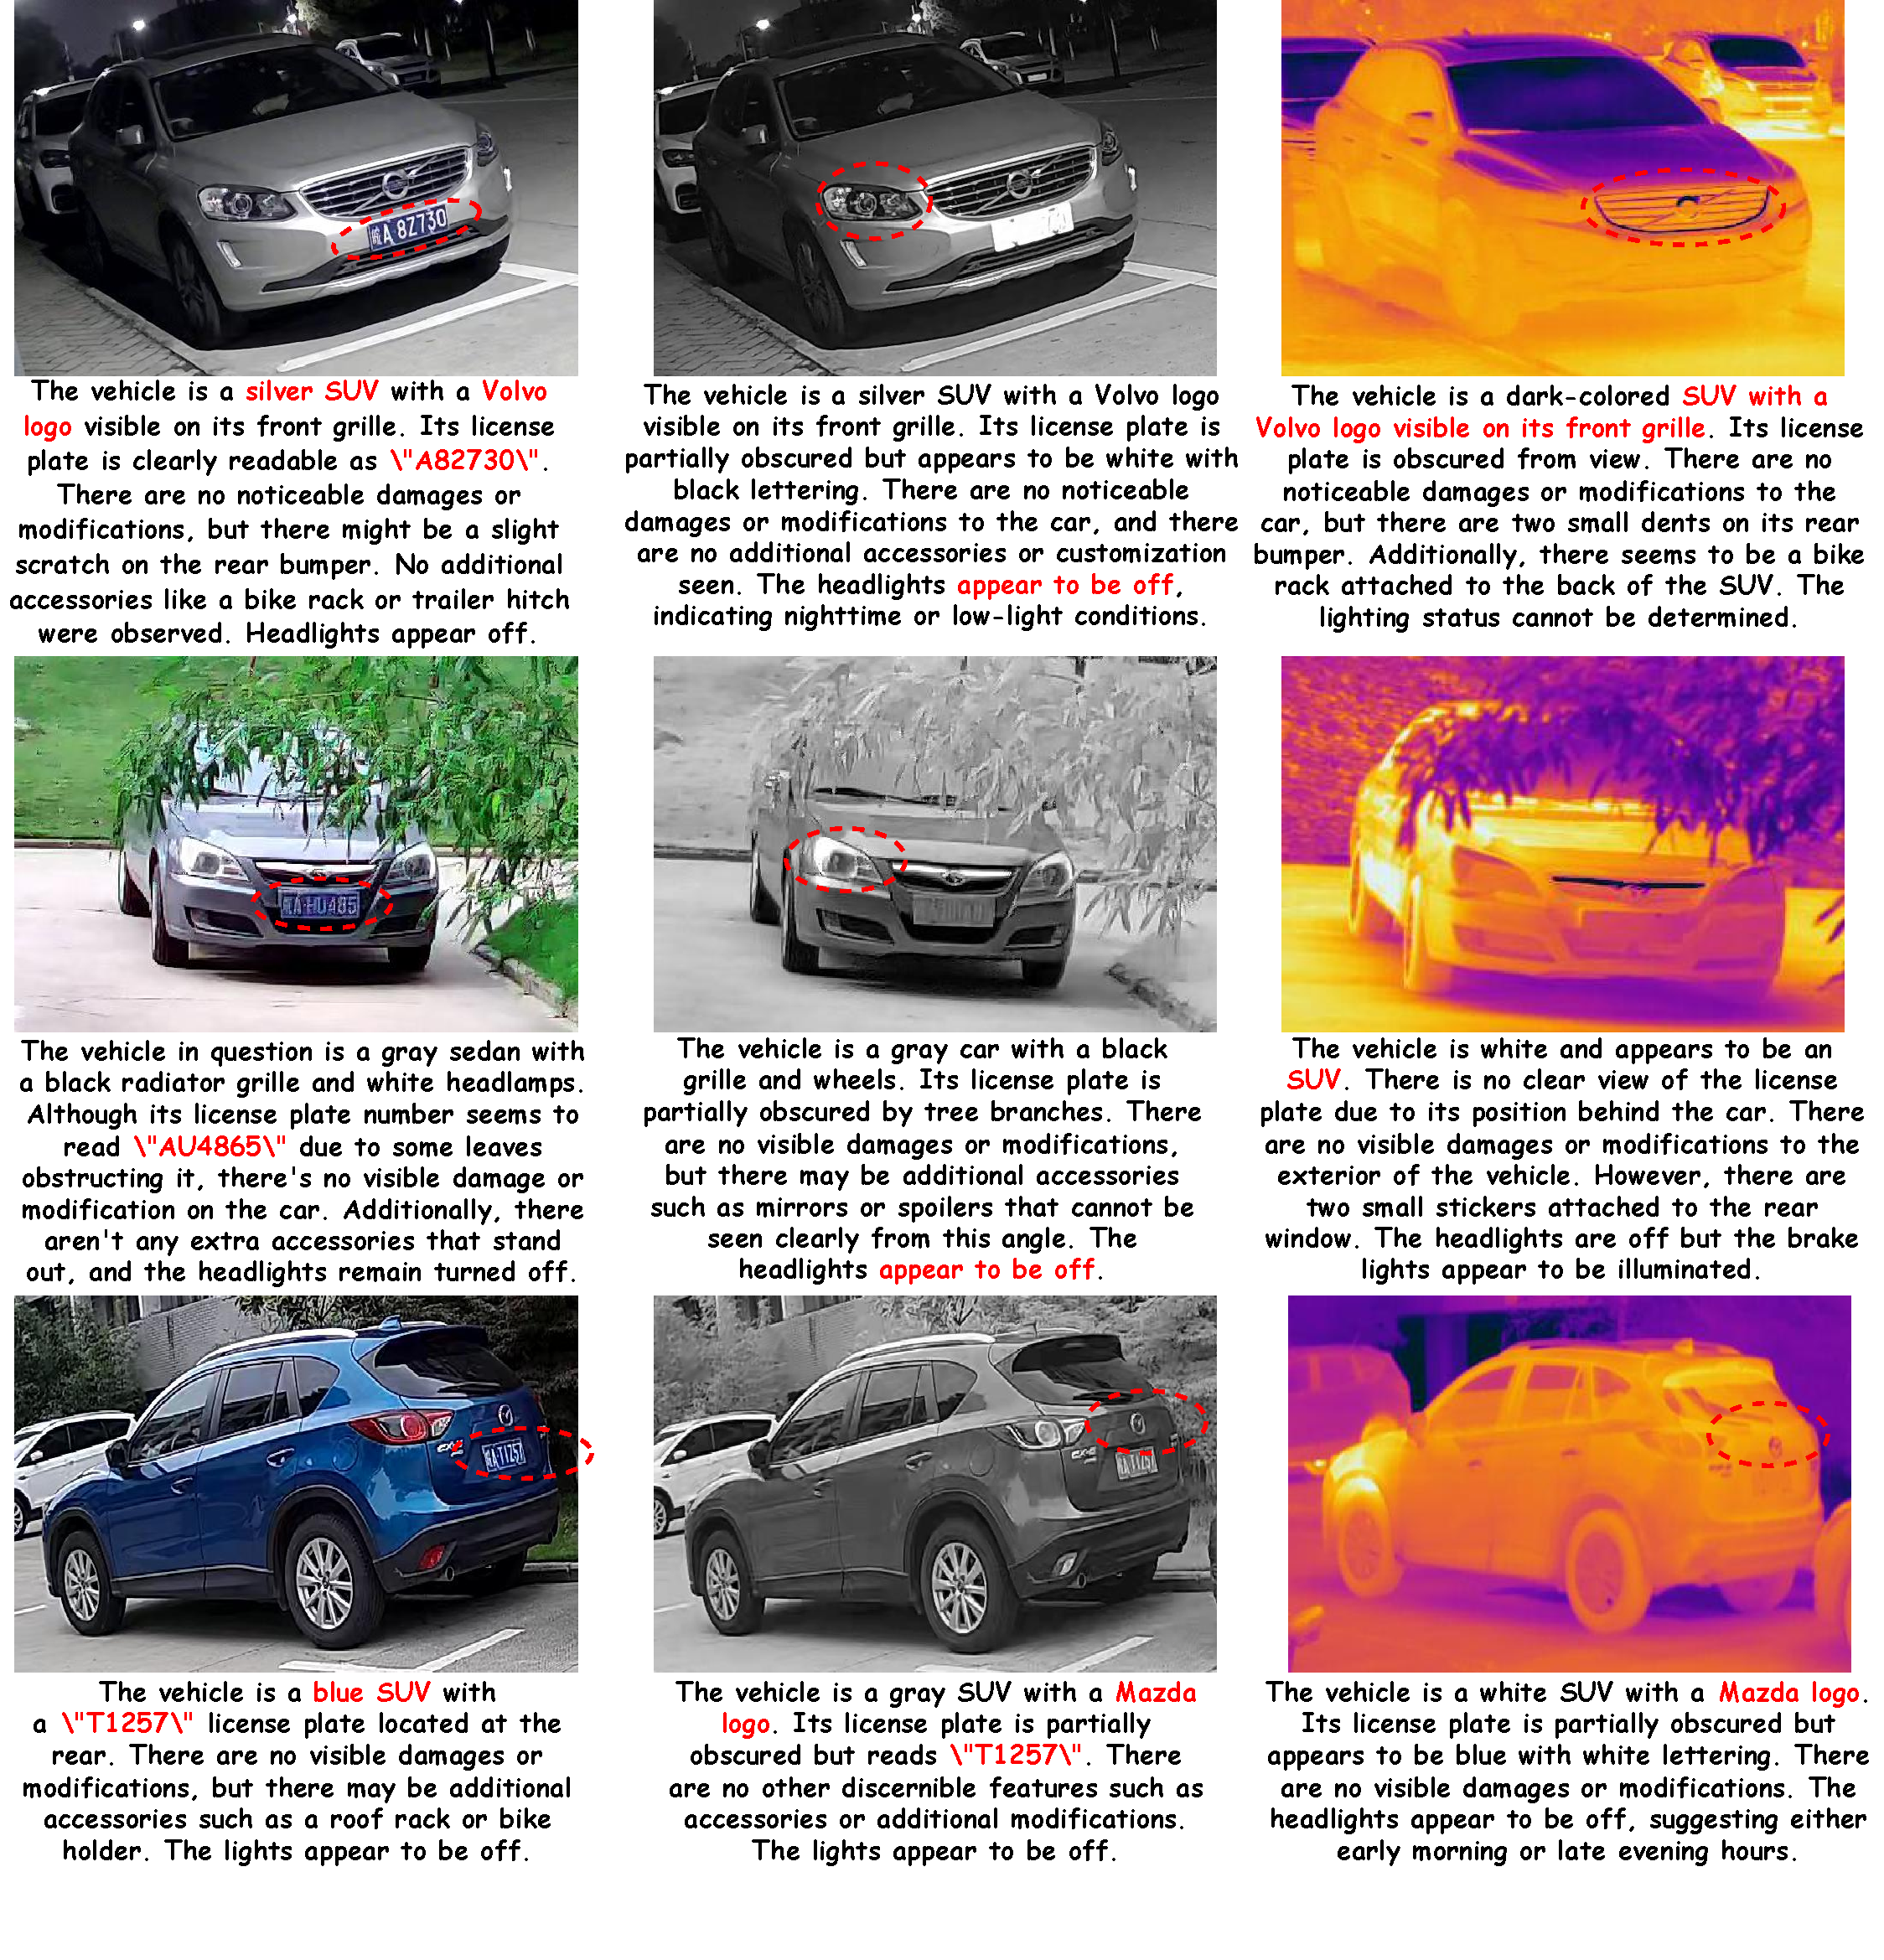
\includegraphics[width=1.\linewidth]{sec/supp_img/More_Instance_Vehicle.pdf}
  }
  \vspace{-2mm}
   \caption{More examples from the multi-modal vehicle ReID dataset MSVR310.}
  \label{fig:more_instance_vehicle}
  \vspace{-6mm}
\end{figure*}
%~~~~~~~~~~~~~~~~~~~~~~~~~~~~~~~~
\\
\textbf{Attribute Extraction:}
%
During the Caption Generation phase, we generate informative text descriptions for each spectrum. However, due to the inherent randomness of MLLMs during the annotation process, issues such as disorganized structure and overly verbose descriptions persist, even with the use of strict templates during generation.
%
To address these challenges, we initially use regular expressions to extract key information from the sentences. While this approach captures most essential attributes, it struggles with handling diverse and complex sentence structures. Fortunately, MLLMs exhibit robust capabilities in extracting key information from text.
%
Leveraging this, we feed the generated descriptions back into the MLLMs with an attribute extraction prompt to specify the predefined attributes to be extracted.
%
The extracted information is then mapped into the template we use in the caption generation phase:
\begin{quote}
  \small
\textit{“Extract the key attributes from the sentence I give you and fill them into the following template: The \{Gender\} is wearing a \{Upper\_Color\} \{Upper\_Garment\} with \{Lower\_Color\} \{Lower\_Garment\} and \{Shoe\_Color\} \{Shoes\}. The \{Gender\} has \{Hairstyle\} \{Hair\_Color\} hair and appears to be \{Age\_Group\}. The \{Gender\} is carrying \{Belongings\}. Strictly follow the template, do not add any extra information."}
\end{quote}
%
This process ensures the generation of concise and informative textual descriptions, effectively mitigating the inconsistencies introduced during the initial phase.
\subsection{More Examples from Different Datasets}
\textbf{Multi-modal Person ReID Dataset Examples.}
%
In \textcolor{red}{Fig.}~\ref{fig:more_instance_person}, we present additional examples from the RGBNT201 dataset to demonstrate the effectiveness of our caption generation pipeline.
%
The generated text descriptions provide rich and informative attributes for each spectrum, including clothing, hairstyle and belongings.
%
These examples verify the effectiveness of our multi-modal captioning pipeline in producing detailed descriptions, which are crucial for multi-modal person ReID under complex visual environments.
%
\\
\textbf{Multi-modal Vehicle ReID Dataset Examples.}
%
In \textcolor{red}{Fig.}~\ref{fig:more_instance_vehicle}, we present additional examples from the MSVR310 dataset to illustrate the effectiveness of our caption generation pipeline in the vehicle ReID scenario.
%
The generated text descriptions capture detailed attributes for each spectrum, including vehicle type, color and license plate number.
%
Notably, descriptions for RGB images reliably provide accurate license plate numbers, while NIR and TIR images focus on attributes such as vehicle type and logo.
%
With these detailed and informative text descriptions, we can fully leverage the semantic information from text descriptions to enhance the performance of multi-modal vehicle ReID.
\section{Details of Modules and Experiments}
\subsection{Details of the Proposed Modules in IDEA}
\textbf{Details of Modal Prefixes.}
To differentiate textual descriptions from various modalities while fine-tuning the CLIP text encoder, we introduce Modal Prefixes.
%
These prefixes consist of two components: a fixed textual description highlighting the characteristics of a specific spectrum and learnable tokens for fine-tuning.
%
This combination enables modality-aware embedding representations.
%
To be specific, the Modal Prefixes for each spectrum are defined as follows:
\begin{itemize}
    \item RGB:
    {\small
    \textit{“An image of a XXXX person in the visible spectrum, capturing natural colors and fine details: "}}
    \item NIR:
    {\small
    \textit{“An image of a XXXX person in the near infrared spectrum, capturing contrasts and surface reflectance: "}}
    \item TIR:
    {\small
    \textit{“An image of a XXXX person in the thermal infrared spectrum, capturing heat emissions as temperature gradients: "}}
\end{itemize}
%
After tokenizing the input text and converting them into embeddings, \textbf{we add randomly initialized learnable tokens} to the embedding at the position corresponding to \textit{“XXXX”}.
%
During fine-tuning, these learnable tokens are updated to capture semantic information among the text descriptions, providing more information for the subsequent InverseNet.
\\
\textbf{Details of InverseNet.}
To fully leverage the semantic information from text descriptions, we propose the InverseNet.
%
Specifically, InverseNet $\mathcal{I}$ is a simple MLP layer that takes the text feature $\hat{f}^{t}_{m}$ as input and outputs a pseudo token ${f}^{t}_{m}$.
%
The input text feature $\hat{f}^{t}_{m}$ is determined based on the presence of learnable tokens in the Modal Prefixes:
\begin{itemize}
    \item If no learnable tokens are added, we directly use the global feature ${f}^{\text{end}}$ from the \textit{“endoftext"} index position of the text, following previous works:
    \begin{equation}
    \hat{f}^{t}_{m} = {f}^{\text{end}}.
    \end{equation}
    \item If learnable tokens are present, we extract the feature corresponding to the position of \textit{“XXXX”}, denoted as ${f}^{\text{prompt}} \in \mathbb{R}^{N_p \times C}$ and average them with ${f}^{\text{end}}$ as follows:
    \begin{equation}
    \hat{f}^{t}_{m} = \frac{1}{N_p + 1} \left( {f}^{\text{end}} + \sum_{i=1}^{N_p} {f}^{\text{prompt}}_i \right).
    \end{equation}
\end{itemize}
%
This approach ensures that the text representation incorporates both the global context from the \textit{“endoftext"} index and the other semantic information provided by the learnable tokens.
%
Then, the pseudo token ${f}^{t}_{m}$ is calculated as follows:
\begin{equation}
    {f}^{t}_{m} = \mathcal{I}(\hat{f}^{t}_{m}) = \omega (\varphi (\omega (\delta (\varphi (\hat{f}^{t}_{m}))))),
\end{equation}
where $\varphi$, $\delta$ and $\omega$ denote the linear layer, GeLU activation function and dropout layer, respectively.
%
Then, the pseudo token ${f}^{t}_{m}$ is concatenated with the visual features, guiding the visual encoder to focus on the interaction between the semantic information and image details.
%
\\
\textbf{Details of CDA.}
To further enhance the interaction between global features and discriminative local information, we propose CDA.
%
In this supplementary material, we clarify the following key points regarding CDA:
%
\begin{itemize}
    \item \textbf{Handling Sampling Point Overflow.}
    During the process of feature extraction, predicted sampling points \(\hat{P}\) may occasionally fall outside the bounds of the feature map.
    %
    To ensure that all sampled locations remain within the valid range, the coordinates are first normalized to the range \([-1, +1]\).
    %
    Subsequently, any sampling point that exceeds this range is clipped to the closest valid value.
    %
    Mathematically, for the sampling point $(\hat{x}, \hat{y})$, the clipping process is defined with the following equations:
    \begin{equation}
    \hat{x} = \text{clip}(\hat{x}, -1, +1), \quad \hat{y} = \text{clip}(\hat{y}, -1, +1).
    \end{equation}
    This clipping process ensures that all coordinates stay within the valid range and allows for stable sampling, particularly at the boundaries of the feature map.

    \item \textbf{Bilinear Interpolation for Feature Sampling.}
    Once the sampling points are determined, we employ bilinear interpolation to extract features from the original feature map \(\hat{F}_m \in \mathbb{R}^{H \times W \times C}\). For each sampling point \((\hat{x}, \hat{y})\), we identify the four neighboring grid points surrounding it.
    %
    Let \((i, j)\) denote the top-left corner of the grid, and the neighboring grid points are then located at \((i+1, j)\), \((i, j+1)\), and \((i+1, j+1)\).
    %
    The interpolation is based on the horizontal and vertical distances between the sampling point \(\hat{P}\) and these neighboring grid points:
    \begin{equation}
    dx = \hat{x} - i, \quad dy = \hat{y} - j.
    \end{equation}
    Then, we calculate the bilinear interpolation weights as:
    \begin{equation}
    w_{mn} = (1 - m \cdot dx)(1 - n \cdot dy), \quad m, n \in \{0, 1\}.
    \end{equation}
    The feature value at the sampled point is then computed as a weighted sum of its neighboring grid points:
    \begin{equation}
      \begin{aligned}
        \hat{F}_m(\hat{x}, \hat{y}) = w_{00}\hat{F}_m(i, j) + w_{10}\hat{F}_m(i+1, j) + \\
        w_{01}\hat{F}_m(i, j+1) + w_{11}\hat{F}_m(i+1, j+1).
      \end{aligned}
  \end{equation}
    This bilinear interpolation procedure ensures that the sampled features are smooth and accurate, effectively preserving discriminative local information.
%
Finally, we get the sampled features from different modalities and reshape them into the token format, which is then concatenated to get \( F_{S} \in \mathbb{R}^{3N_{S} \times C} \), where \( N_{S} = H_{S} \times W_{S} \).
\end{itemize}
With the above details of our proposed modules, we can effectively leverage the semantic information from text descriptions and enhance the interaction between global features and discriminative local information, leading to superior performance in multi-modal object ReID tasks.
\subsection{Details of Models in the Ablation Study}
\textbf{Model B in \textcolor{red}{Tab.}~\ref{tab:main_ablation}.}
%
In \textcolor{red}{Tab.}~\ref{tab:main_ablation} of the main manuscript, Model B integrates text information using a parallel structure.
%
Specifically, this parallel structure is depicted in \textcolor{red}{Fig.}~\ref{fig:inverse_direction} (a), where the text feature is directly concatenated with the visual feature for retrieval.
%
In this configuration, the text information is not utilized as effectively as in IMFE.
\\
\textbf{Model A in \textcolor{red}{Tab.}~\ref{tab:CDA_ablation}.}
%
In \textcolor{red}{Tab.}~\ref{tab:CDA_ablation} of the main manuscript, Model A does not any components in CDA.
%
All the patch tokens from different modalities are directly concatenated to interact with each other using the self-attention mechanism.
%
After the interaction, we pool the features from different modalities and concatenate them for retrieval.
%
Due to the limited local information, the performance of Model A is inferior to the global feature in IMFE.
\\
\textbf{IDEA w/o Text in \textcolor{red}{Tab.}~\ref{tab:Text_ablation}.}
%
To evaluate the importance of text information in IDEA, we compare the performance of IDEA with and without text information in \textcolor{red}{Tab.}~\ref{tab:Text_ablation}.
%
In fact, our IDEA can also work without text information.
%
Under this setting, our IDEA is composed of \textbf{the visual baseline and the CDA}, which only utilizes visual information for retrieval.
%
The results show that the text information significantly enhances the performance of IDEA, demonstrating the importance of leveraging semantic guidance.
\\
\textbf{IDEA w/o Offset in \textcolor{red}{Tab.}~\ref{tab:Offset_ablation}.}
%
In \textcolor{red}{Tab.}~\ref{tab:Offset_ablation}, we assess the effectiveness of the offset mechanism in CDA.
%
When the offset is not used, we rely on convolutional layers to process \( \hat{F}_{m} \), generating features that aggregate local information, which are of the same shape as our \( F_{S} \).
%
The results demonstrate that the offset mechanism enhances the capture of discriminative local information, leading to improved performance.
\begin{figure}[t]
  \centering
    \resizebox{0.475\textwidth}{!}
    {
  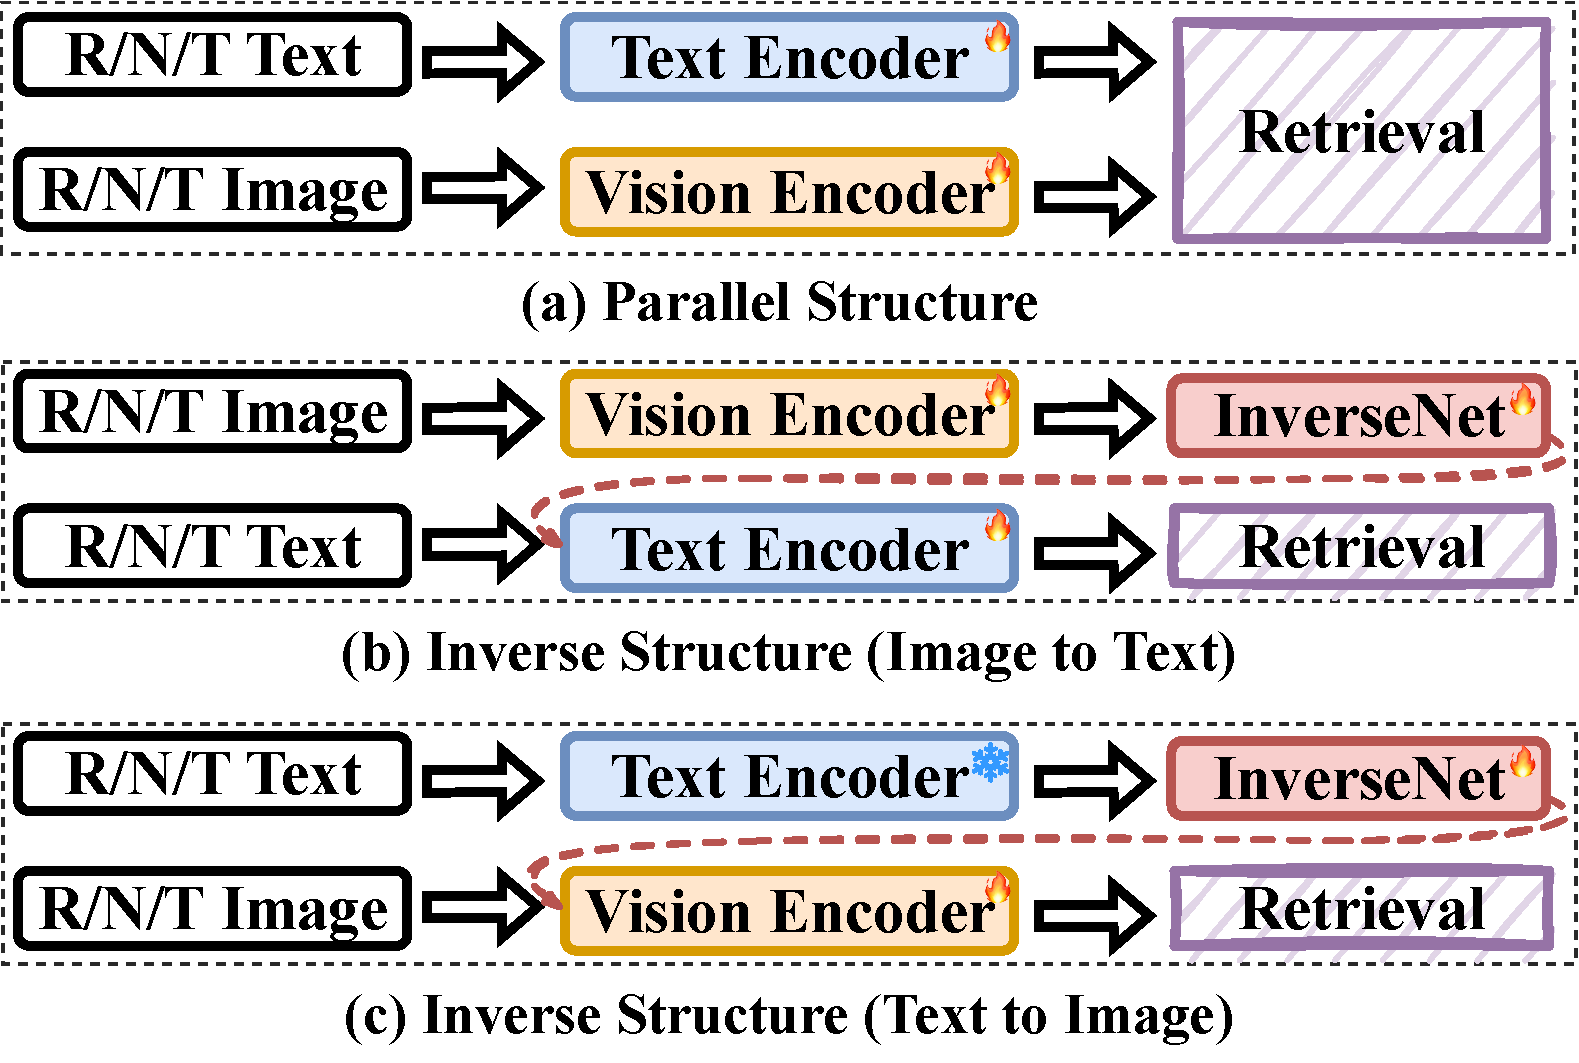
\includegraphics[width=30\linewidth]{sec/supp_img/Comparision_Parrel.pdf}
  }
  \vspace{-4mm}
   \caption{Comparison of different structures in the IMFE.}
  \label{fig:inverse_direction}
  \vspace{-2mm}
\end{figure}
\begin{table}[t]
  \centering
  \renewcommand\arraystretch{1.2}
  \setlength\tabcolsep{1.5pt}
  \resizebox{0.478\textwidth}{!}
  {
  \begin{tabular}{ccccccccc}
    \noalign{\hrule height 1pt}
    \multicolumn{1}{c}{\multirow{2}{*}{\textbf{Methods}}} &\multicolumn{1}{c}{\multirow{1}{*}{\textbf{Params}}} &  \multicolumn{2}{c}{\textbf{RGBNT201}} &  \multicolumn{2}{c}{\textbf{RGBNT100}} & \multicolumn{2}{c}{\textbf{MSVR310}} \\
    \cmidrule(r){2-2} \cmidrule(r){3-4} \cmidrule(r){5-6} \cmidrule(r){7-8}
    &\textbf{M} & \textbf{mAP} & \textbf{R-1}& \textbf{mAP} & \textbf{R-1} &\textbf{mAP} & \textbf{R-1} \\
    \hline
  HAMNet~\cite{li2020multi} &  78.00 &27.7 &26.3 &74.5 &93.3 &27.1 &42.3\\
  CCNet~\cite{zheng2023cross} &  74.60 &- &- & 77.2 &96.3 &36.4 &55.2\\
  IEEE~\cite{wang2022interact} & 109.22 &49.5&48.4 &-&-&-&-\\
  GAFNet~\cite{guo2022generative} &  130.00 &- &- &74.4 &93.4 &- &-\\
  \hline
  UniCat$^*$~\cite{crawford2023unicat}  & 259.02 &57.0 &55.7&79.4&96.2&- &- \\
  GraFT$^*$~\cite{yin2023graft} & 101.00 &- &- &76.6&94.3&-&-\\
  TOP-ReID$^*$~\cite{wang2024top} & 324.53 &72.3 &76.6 &81.2&96.4&35.9&44.6\\
  EDITOR$^*$~\cite{zhang2024magic} &118.55 & 66.5       & 68.3& 82.1 & 96.4 &39.0 & 49.3\\
  RSCNet$^*$~\cite{yu2024representation} &  124.10 & 68.2 & 72.5 &82.3 &\underline{96.6} &39.5 &49.6\\
  WTSF-ReID$^*$~\cite{yu2025wtsf} &  143.60 & 67.9 & 72.2 & 82.2 &96.5 &39.2 &49.1\\
  MambaPro$\dagger$~\cite{wang2024mambapro} & 74.20 &78.9&\textbf{83.4}&83.9 &94.7 & \underline{47.0} &56.5\\
  DeMo$\dagger$~\cite{wang2024decoupled} & 98.79 &\underline{79.0}&\underline{82.3}&\underline{86.2} &\textbf{97.6} & \textbf{49.2} &\underline{59.8}\\
  \hline
  \rowcolor[gray]{0.92}
  IDEA$\dagger$ & 91.67 &\textbf{80.2}&82.1&\textbf{87.2} &96.5 & \underline{47.0} &\textbf{62.4}\\
  \noalign{\hrule height 1pt}
  \end{tabular}
  }
  \vspace{-2mm}
  \caption{Parameter and performance comparison with state-of-the-art methods.
  %
  The best and second results are in bold and underlined, respectively.
  %
  The symbol $\dagger$ denotes CLIP-based methods, $*$ indicates ViT-based methods and others are CNN-based methods.}
  \label{tab:params}
  \vspace{-2mm}
  \end{table}
%~~~~~~~~~~~~~~~~~~~~~~~~~~~~~~~~~~~~~~~~~~~~~~~~~~~~~~~~~~~~~~~~~~~~~~~~~~~~~~~~~~~~~~~~~~~~~~~
\section{Module Validation and Analysis}
\textbf{Analysis of Model Parameters and Performance.}
In \textcolor{red}{Tab.}~\ref{tab:params}, we compare the trainable parameters and performance of our proposed IDEA model with several state-of-the-art methods, including CNN-based approaches and Transformer-based techniques.
%
While Transformer-based methods typically have more parameters than CNN-based approaches, they often deliver superior performance due to their strong generalization capabilities.
%
Among these, our proposed IDEA stands out by achieving state-of-the-art performance with significantly fewer parameters.
%
For instance, IDEA requires only 91.67M parameters, far less than TOP-ReID’s 324.53M, yet it achieves substantial improvements in mAP and Rank-1 accuracy.
%
On the RGBNT201 dataset, IDEA achieves an mAP of 80.2\%, surpassing the previous best of 79.0\% mAP by DeMo.
%
Similarly, on the RGBNT100 dataset, IDEA achieves an mAP of 87.2\%, which is 1\% higher than DeMo.
%
These results demonstrate the effectiveness and efficiency of our proposed IDEA.
\begin{table}[t]
  \centering
  \renewcommand\arraystretch{1.1}
  \setlength\tabcolsep{4.5pt}
  \resizebox{0.475\textwidth}{!}
  {
  \begin{tabular}{cccccc}
      \noalign{\hrule height 1pt}
      \multicolumn{1}{c}{\multirow{2}{*}{\textbf{Index}}} &\multirow{2}{*}{\textbf{Inverse Direction}} & \multicolumn{4}{c}{\textbf{Metrics}} \\
      \cmidrule(r){3-6}
          &   & \textbf{mAP}    & \textbf{Rank-1}   & \textbf{Rank-5} & \textbf{Rank-10} \\\hline
  \multirow{1}{*}{A} & Image to Text   &\underline{72.0}  &\underline{73.4} &\underline{83.4}  &\underline{89.2}\\
  \rowcolor[gray]{0.92}
  \multirow{1}{*}{B} & Text to Image    &\textbf{77.2} &\textbf{81.1}  &\textbf{88.4} &\textbf{92.2}\\
  \noalign{\hrule height 1pt}
  \end{tabular}
  }
  \vspace{-2mm}
  \caption{Comparison of inverse directions on RGBNT201.}
  \label{tab:image_inverse}
  \vspace{-2mm}
\end{table}
%~~~~~~~~~~~~~~~~~~~~~~~~~~~~~~~~~~~~~~~~~~~~~~~~~~~~~~~~~~~~~~~~~~~~~~~~~~~~~~~~~~~~~~~~~~~~~~~
\\
\textbf{Comparison with Different Inverse Directions.}
To further validate the effectiveness of our proposed IMFE, we compare the performance of IDEA using different inverse directions on the RGBNT201 dataset.
%
As shown in \textcolor{red}{Tab.}~\ref{tab:image_inverse}, Model B in \textcolor{red}{Fig.}~\ref{fig:inverse_direction} (c) outperforms Model A in \textcolor{red}{Fig.}~\ref{fig:inverse_direction} (b), achieving an mAP of 77.2\% and Rank-1 accuracy of 81.1\%, compared to 72.0\% mAP and 73.4\% Rank-1 accuracy for the image-to-text direction.
%
These findings highlight the importance of leveraging semantic guidance from text descriptions to enrich visual interactions.
%
However, the inherent limitations of multi-modal captioning, where the text modality serves as the primary fusion source, may introduce inconsistencies across spectra, resulting in a performance drop in certain cases.
%
Thus, we adopt the text-to-image direction in our IDEA model as default setting.
\\
\textbf{Comparison with CLIP-based TOP-ReID.}
In \textcolor{red}{Tab.}~\ref{tab:pre}, we compare our IDEA model with TOP-ReID~\cite{wang2024top}, both utilizing the CLIP vision encoder.
%
IDEA consistently outperforms TOP-ReID on the RGBNT201 dataset, achieving an mAP of 80.2\% and Rank-1 accuracy of 82.1\%, compared to TOP-ReID’s 73.3\% mAP and 77.2\% Rank-1 accuracy.
%
These results highlight the effectiveness of our proposed modules in fully leveraging CLIP's knowledge.
\begin{table}[t]
  \vspace{-0mm}
  \centering
  \renewcommand\arraystretch{1.1}
  \setlength\tabcolsep{4.5pt}
  \resizebox{0.475\textwidth}{!}
  {
  \begin{tabular}{cccccc}
    \noalign{\hrule height 1pt}
  {\multirow{2}{*}{\textbf{Methods}}} &{\multirow{1}{*}{\textbf{Params}}}&  \multicolumn{4}{c}{\textbf{Metrics}} \\
  \cmidrule(r){2-2} \cmidrule(r){3-6}
  &\textbf{M} & \textbf{mAP} & \textbf{Rank-1} & \textbf{Rank-5} & \textbf{Rank-10} \\\hline
    TOP-ReID (CLIP) & \multirow{1}{*}{324.53} &\underline{73.3} &\underline{77.2} &\underline{85.9} &\underline{90.1}  \\
    \rowcolor[gray]{0.92}
    IDEA &\multirow{1}{*}{91.67}    &\textbf{80.2} &\textbf{82.1} &\textbf{90.0} &\textbf{93.3}  \\
  \noalign{\hrule height 1pt}
  \end{tabular}
  }
  \vspace{-2mm}
  \caption{Comparison with TOP-ReID (CLIP) on RGBNT201.}
  \vspace{-2mm}
  \label{tab:pre}
\end{table}
\begin{table}[t]
  \centering
  \renewcommand\arraystretch{1.1}
 \setlength\tabcolsep{4.5pt}
  \resizebox{0.475\textwidth}{!}
  { % 
      \begin{tabular}{ccccc}
        \noalign{\hrule height 1pt}
      \textbf{Model} & \textbf{Training Time (h)} & \textbf{Memory (GB)} & \textbf{Time per Epoch (min)} & \textbf{Samples/s} \\
      \midrule
      TOP-ReID     & 0.6650              & 17.80            & 0.3325          & 168.03           \\
      EDITOR       & 0.4074                 & 16.41               & 0.3492              & 167.01             \\
      \rowcolor[gray]{0.92}
      \textbf{IDEA}         & \textbf{0.3075}             & \textbf{18.02}            & \textbf{0.3600}           & \textbf{159.68}           \\
      \noalign{\hrule height 1pt}
      \end{tabular}
  }
  \vspace{-2mm}
  \caption{Training efficiency comparison on RGBNT201.}
  \vspace{-2mm}
  \label{tab:efficiency}
\end{table}
%~~~~~~~~~~~~~~~~~~~~~~~~~~~~~~~~~~~~~~~~~~~~~~~~~~~~~~~~~~~~~~~~~~~~~~~~~~~~~~~~~~~~~~~~~~~~~~~
\\
\textbf{Training Efficiency Comparison.}
As shown in \textcolor{red}{Tab.}~\ref{tab:efficiency}, IDEA demonstrates competitive training efficiency.
%
Moreover, it requires \textbf{less time to converge}, benefiting from the effective utilization of semantic information from text descriptions.
%
This guidance enables the model to focus on discriminative local features, accelerating convergence.
%
Furthermore, GPU memory usage remains \textbf{below 24GB} during both training and inference.
%
On the smaller RGBNT201 dataset, training can be completed \textbf{within 20 minutes}, further highlighting the efficiency of our proposed IDEA.
\\
\textbf{Effect of Text with Different Modalities Combination.}
In \textcolor{red}{Tab.}~\ref{tab:textIR}, we compare the performance of different modality combinations on the RGBNT201 dataset.
%
Here, \textbf{R} refers to the RGB image modality along with text annotations derived from RGB images, while \textbf{N} and \textbf{T} represent the NIR and TIR image-text pairs, respectively.
%
A crucial aspect of multi-modal object ReID is effectively integrating complementary information across modalities.
%
Even with the addition of textual annotations, multi-spectral information remains indispensable.
%
As shown in \textcolor{red}{Tab.}~\ref{tab:textIR}, incorporating IR data significantly enhances performance, underscoring its critical role in capturing essential identity cues.
%
The results highlight that while text provides valuable semantic guidance, it cannot fully replace the rich visual and spectral details contributed by multi-modal fusion.
\begin{table}[t]
    \centering
    \renewcommand\arraystretch{1.1}
   \setlength\tabcolsep{4.5pt}
    \resizebox{0.475\textwidth}{!}
    { % 
        \begin{tabular}{cccccccc}
          \noalign{\hrule height 1pt}
        \textbf{Modality} &\textbf{R} & \textbf{N} & \textbf{T} & \textbf{R+N} & \textbf{R+T}& \textbf{N+T}& \textbf{R+N+T} \\
        \midrule
        mAP &39.9      & 27.1       &43.3& 58.4 & 71.5         & 62.9               & 80.2                     \\
        \noalign{\hrule height 1pt}
        \end{tabular}
    }
    \caption{\small Comparison of modalities combination on RGBNT201.}
    \label{tab:textIR}
\end{table}
\\
%~~~~~~~~~~~~~~~~~~~~~~~~~~~~~~~~~~~~~~~~~~~~~~~~~~~~~~~~~~~~~~~~~~~~~~~~~~~~~~~~~~~~~~~~~~~~~~~
\textbf{Exploration of Extreme Cases with Missing Text.}
In \textcolor{red}{Tab.}~\ref{tab:textMissing}, we explore the impact of missing text annotations during retrieval on the RGBNT201 dataset.
%
Notably, in the most extreme case where all text annotations are removed, IDEA still achieves a mAP of 79.5\%, which is only a marginal drop from the fully annotated setting.
%
This indicates that during training, the semantic guidance provided by text effectively enhances the fusion between multi-modal features, enabling the model to learn more robust representations.
%
These findings validate that IDEA does not excessively rely on textual input during inference but instead leverages structured multi-modal learning to develop a more robust and adaptive feature representation.
\begin{table}[t]
  \centering
  \renewcommand\arraystretch{1.1}
   \setlength\tabcolsep{4.5pt}
  \resizebox{0.475\textwidth}{!}
  { % 
      \begin{tabular}{ccccccccc}
        \noalign{\hrule height 1pt}
      \textbf{Cases} &\textbf{Full} & \textbf{M(R)} & \textbf{M(N)} & \textbf{M(T)} & \textbf{M(RN)}& \textbf{M(RT)}& \textbf{M(NT)}& \textbf{M(RNT)} \\
      \midrule
      mAP &80.2       & 79.8       &80.0& 79.9 & 79.7         & 79.6               & 79.8              & 79.5             \\
      \noalign{\hrule height 1pt}
      \end{tabular}
  }
  \caption{Comparison of text-missing cases on RGBNT201.
  %
  M(X) indicates that the text annotations for modality X are blank strings.}
  \label{tab:textMissing}
\end{table}
\begin{table}[t]
  \centering
  \renewcommand\arraystretch{1.}
  \setlength\tabcolsep{4.5pt}
  \resizebox{0.35\textwidth}{!}
  {
  \begin{tabular}{cccccc}
      \noalign{\hrule height 1pt}
      \multicolumn{1}{c}{\multirow{2}{*}{\textbf{Index}}} &\multicolumn{3}{c}{\textbf{Modules}} & \multicolumn{2}{c}{\textbf{Metrics}} \\
      \cmidrule(r){2-4} \cmidrule(r){5-6}
 & \textbf{Text}              & \textbf{IMFE}                & \textbf{CDA}                   & \textbf{mAP}    & \textbf{Rank-1}   \\\hline
  A                  & \ding{53}                  & \ding{53}                  & \ding{53}                    & 40.4  & 56.0 \\
  B                  & \ding{51}                  & \ding{53}                  & \ding{53}                      & 43.5  & 57.9 \\
  \multirow{1}{*}{C} & \multirow{1}{*}{\ding{51}} & \multirow{1}{*}{\ding{51}} & \multirow{1}{*}{\ding{53}}    & \underline{45.7}  & \underline{61.1} \\
  \rowcolor[gray]{0.92}
  \multirow{1}{*}{D} & \multirow{1}{*}{\ding{51}} & \multirow{1}{*}{\ding{51}} & \multirow{1}{*}{\ding{51}}    &\textbf{47.0} &\textbf{62.4}  \\
  \noalign{\hrule height 1pt}
  \end{tabular}
  }
  \vspace{-2mm}
  \caption{Comparison with different modules on MSVR310.}
  \label{tab:main_ablation_vehicle}
  \vspace{-6mm}
\end{table}
%~~~~~~~~~~~~~~~~~~~~~~~~~~~~~~~~~~~~~~~~~~~~~~~~~~~~~~~~~~~~~~~~~~~~~~~~~~~~~~~~~~~~~~~~~~~~~~~
\\
\textbf{Effect of Key Modules on Vehicle Dataset.}
In \textcolor{red}{Tab.}~\ref{tab:main_ablation_vehicle}, we present the performance comparison of different modules on the MSVR310 vehicle dataset.
%
Model A, which only uses visual information, achieves an mAP of 40.4\% and Rank-1 accuracy of 56.0\%.
%
Model B introduces the text information with a parallel structure, leading to a 3.1\% improvement in mAP compared to Model A.
%
Model C further incorporates the IMFE, which fully leverages the semantic guidance from the text, resulting in a 2.2\% improvement in mAP.
%
Finally, Model D integrates the CDA, leading to a 1.3\% improvement in mAP compared to Model C, achieving the best performance with an mAP of 47.0\% and Rank-1 accuracy of 62.4\%.
%
These results fully validate the effectiveness and efficiency of our proposed modules.
\\
\textbf{Hyper-parameter Analysis for Vehicle Dataset.}
\textcolor{red}{Fig.}~\ref{fig:prompt_offset_msvr310} presents a performance comparison across different prompt lengths and offset factors on the MSVR310 vehicle dataset.
%
The results demonstrate a general performance improvement with increasing prompt length.
%
However, performance begins to decline when the prompt length exceeds 1.
%
Consequently, we adopt a prompt length of 1 for subsequent experiments on MSVR310.
%
A similar observation holds for the RGBNT201 dataset, where longer prompts truncate text descriptions, leading to the loss of critical information.
%
For the offset factor, the performance remains relatively stable, with the optimal result achieved at an offset factor of 25.
\begin{figure}[t]
  \centering
    \resizebox{0.475\textwidth}{!}
    {
  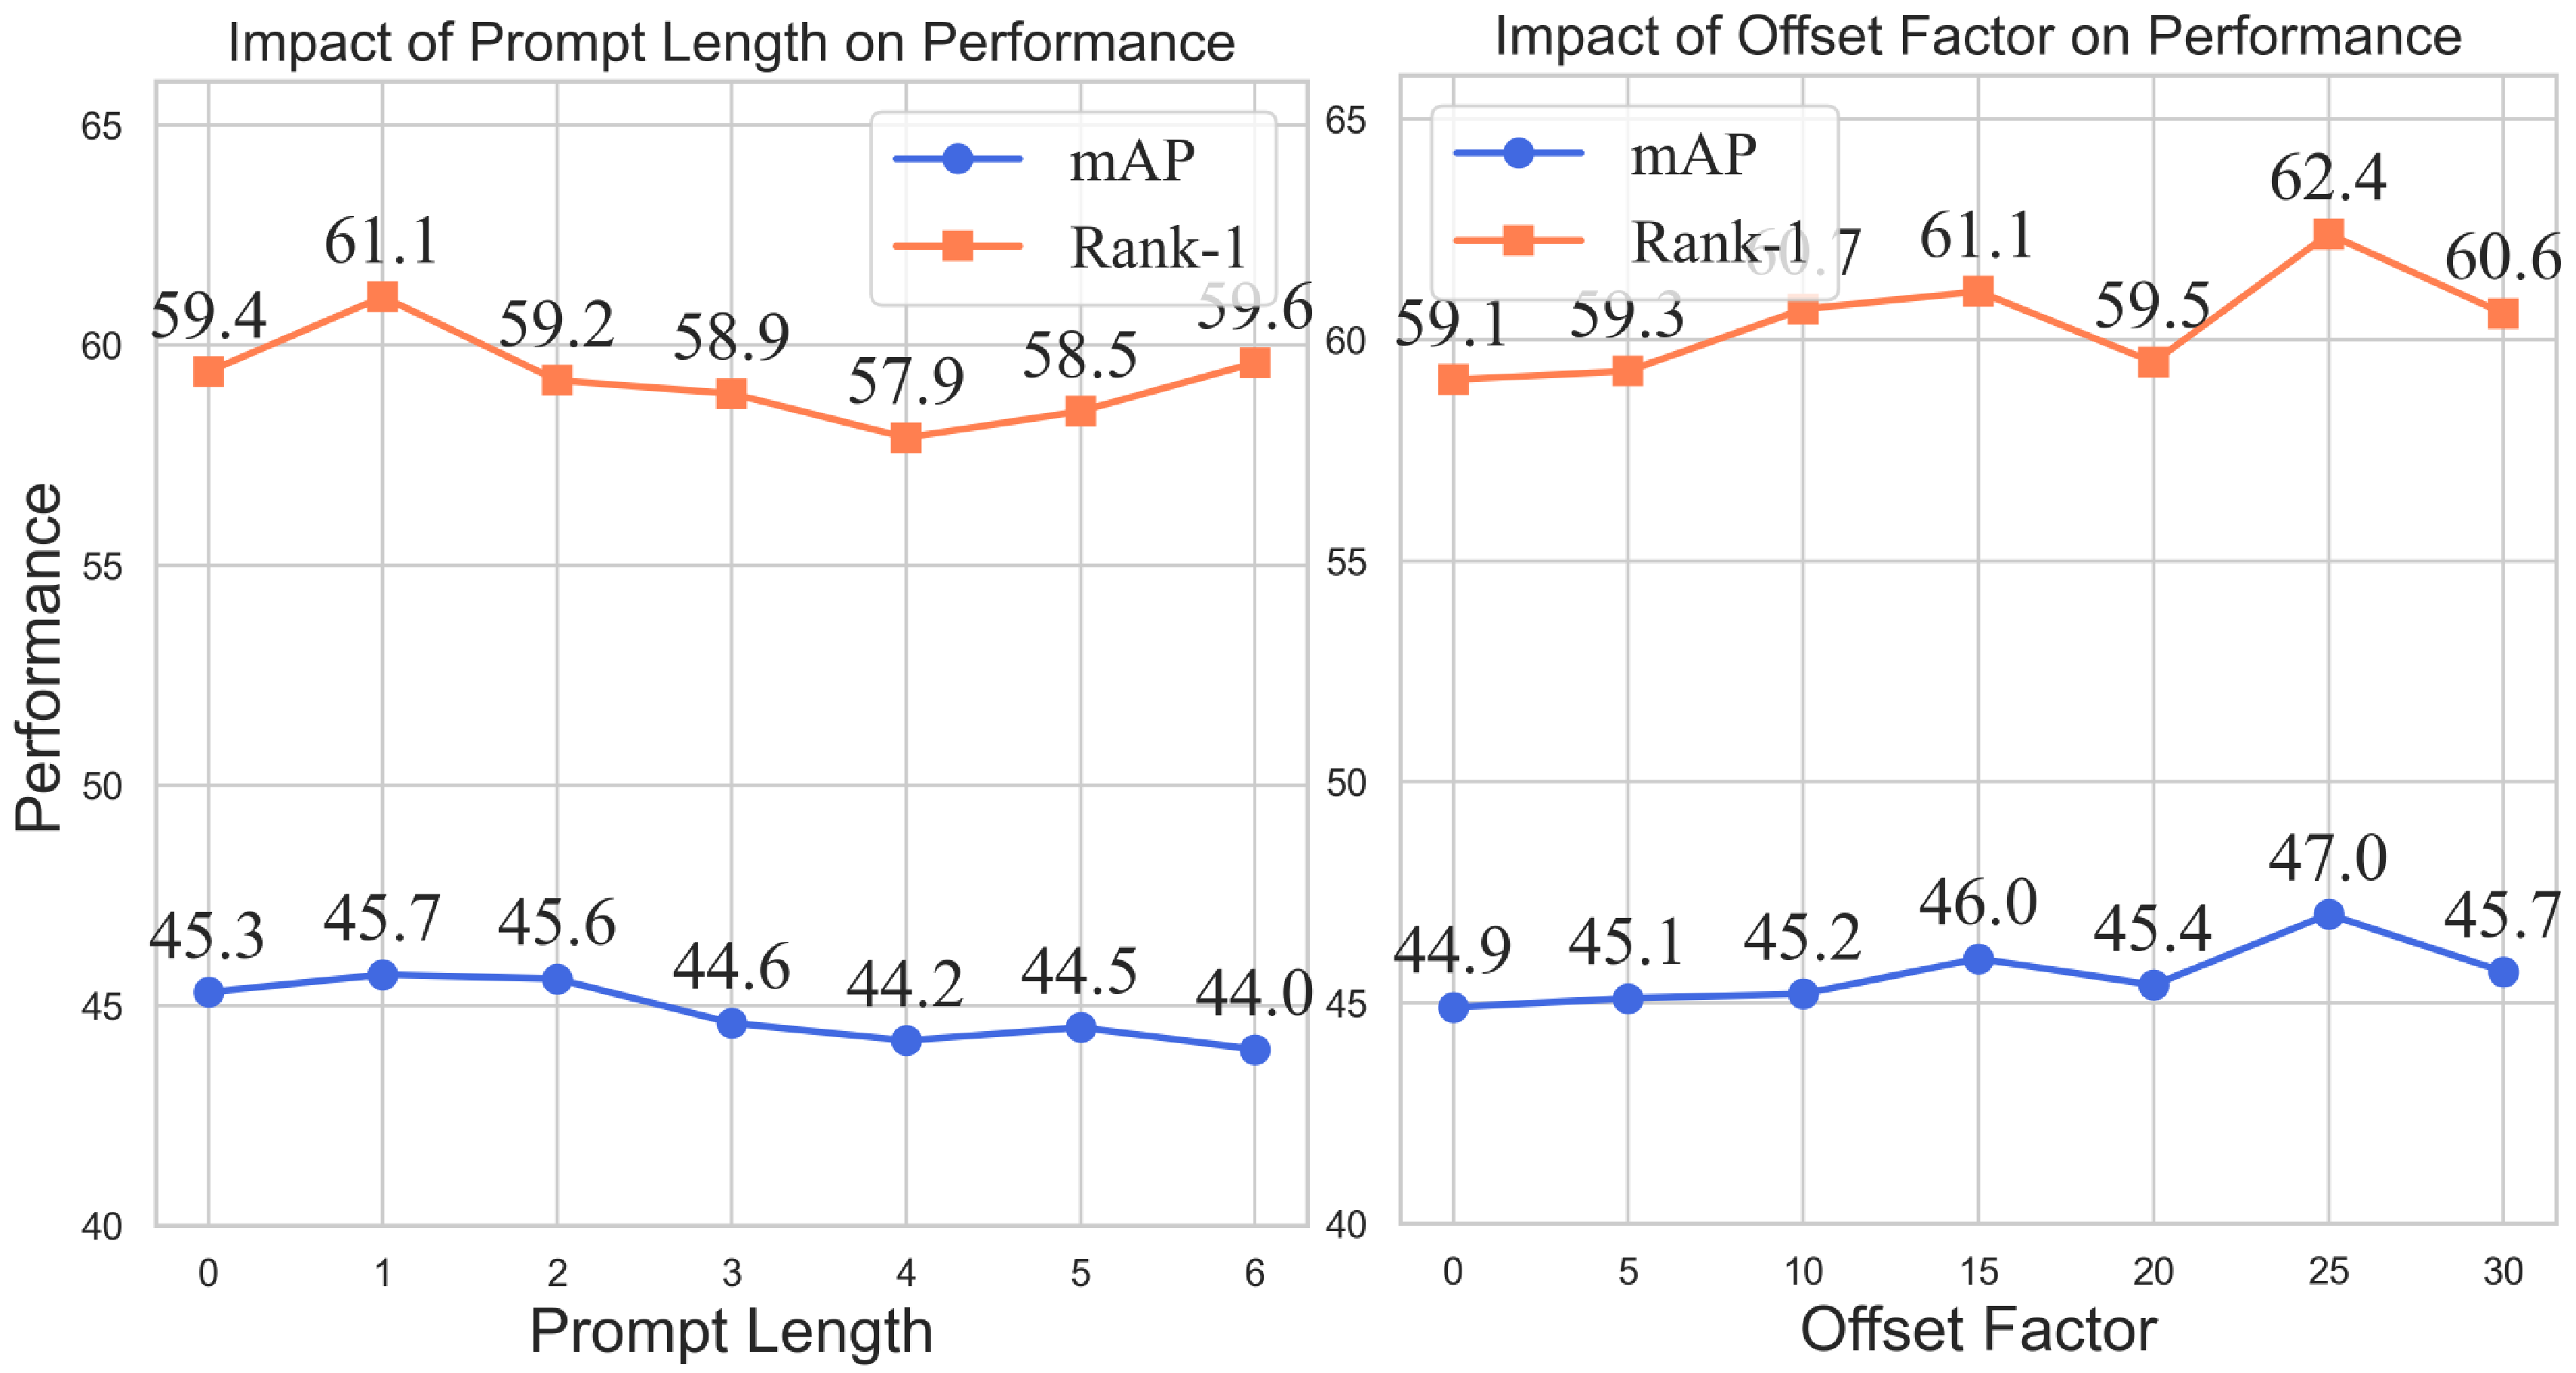
\includegraphics[width=30\linewidth]{sec/supp_img/Hyper_MSVR310.pdf}
  }
  \vspace{-3mm}
   \caption{Performance comparison with different prompt lengths and offset factors on multi-modal vehicle dataset MSVR310.}
  \label{fig:prompt_offset_msvr310}
  \vspace{-6mm}
\end{figure}
%~~~~~~~~~~~~~~~~~~~~~~~~~~~~~~~~
\section{Visualization Analysis of IDEA}
\subsection{More Visualization for Person ReID}
\textbf{Visualization of Channel Activation Maps on the Person ReID Dataset.}
\textcolor{red}{Fig.}~\ref{fig:channel_act} illustrates the channel activation maps across different modalities for person ReID datasets within our IDEA framework.
%
Each modality exhibits distinct activation patterns, reflecting their unique spectral properties.
%
Notably, these maps successfully identify semantic regions, including hair, clothing and accessories, underscoring the capability of our proposed modules to effectively leverage multi-modal information.
\\
\textbf{Visualization of Multi-modal Ranking List with Different Modules in IDEA.}
\begin{figure}[t]
  \centering
    \resizebox{0.475\textwidth}{!}
    {
  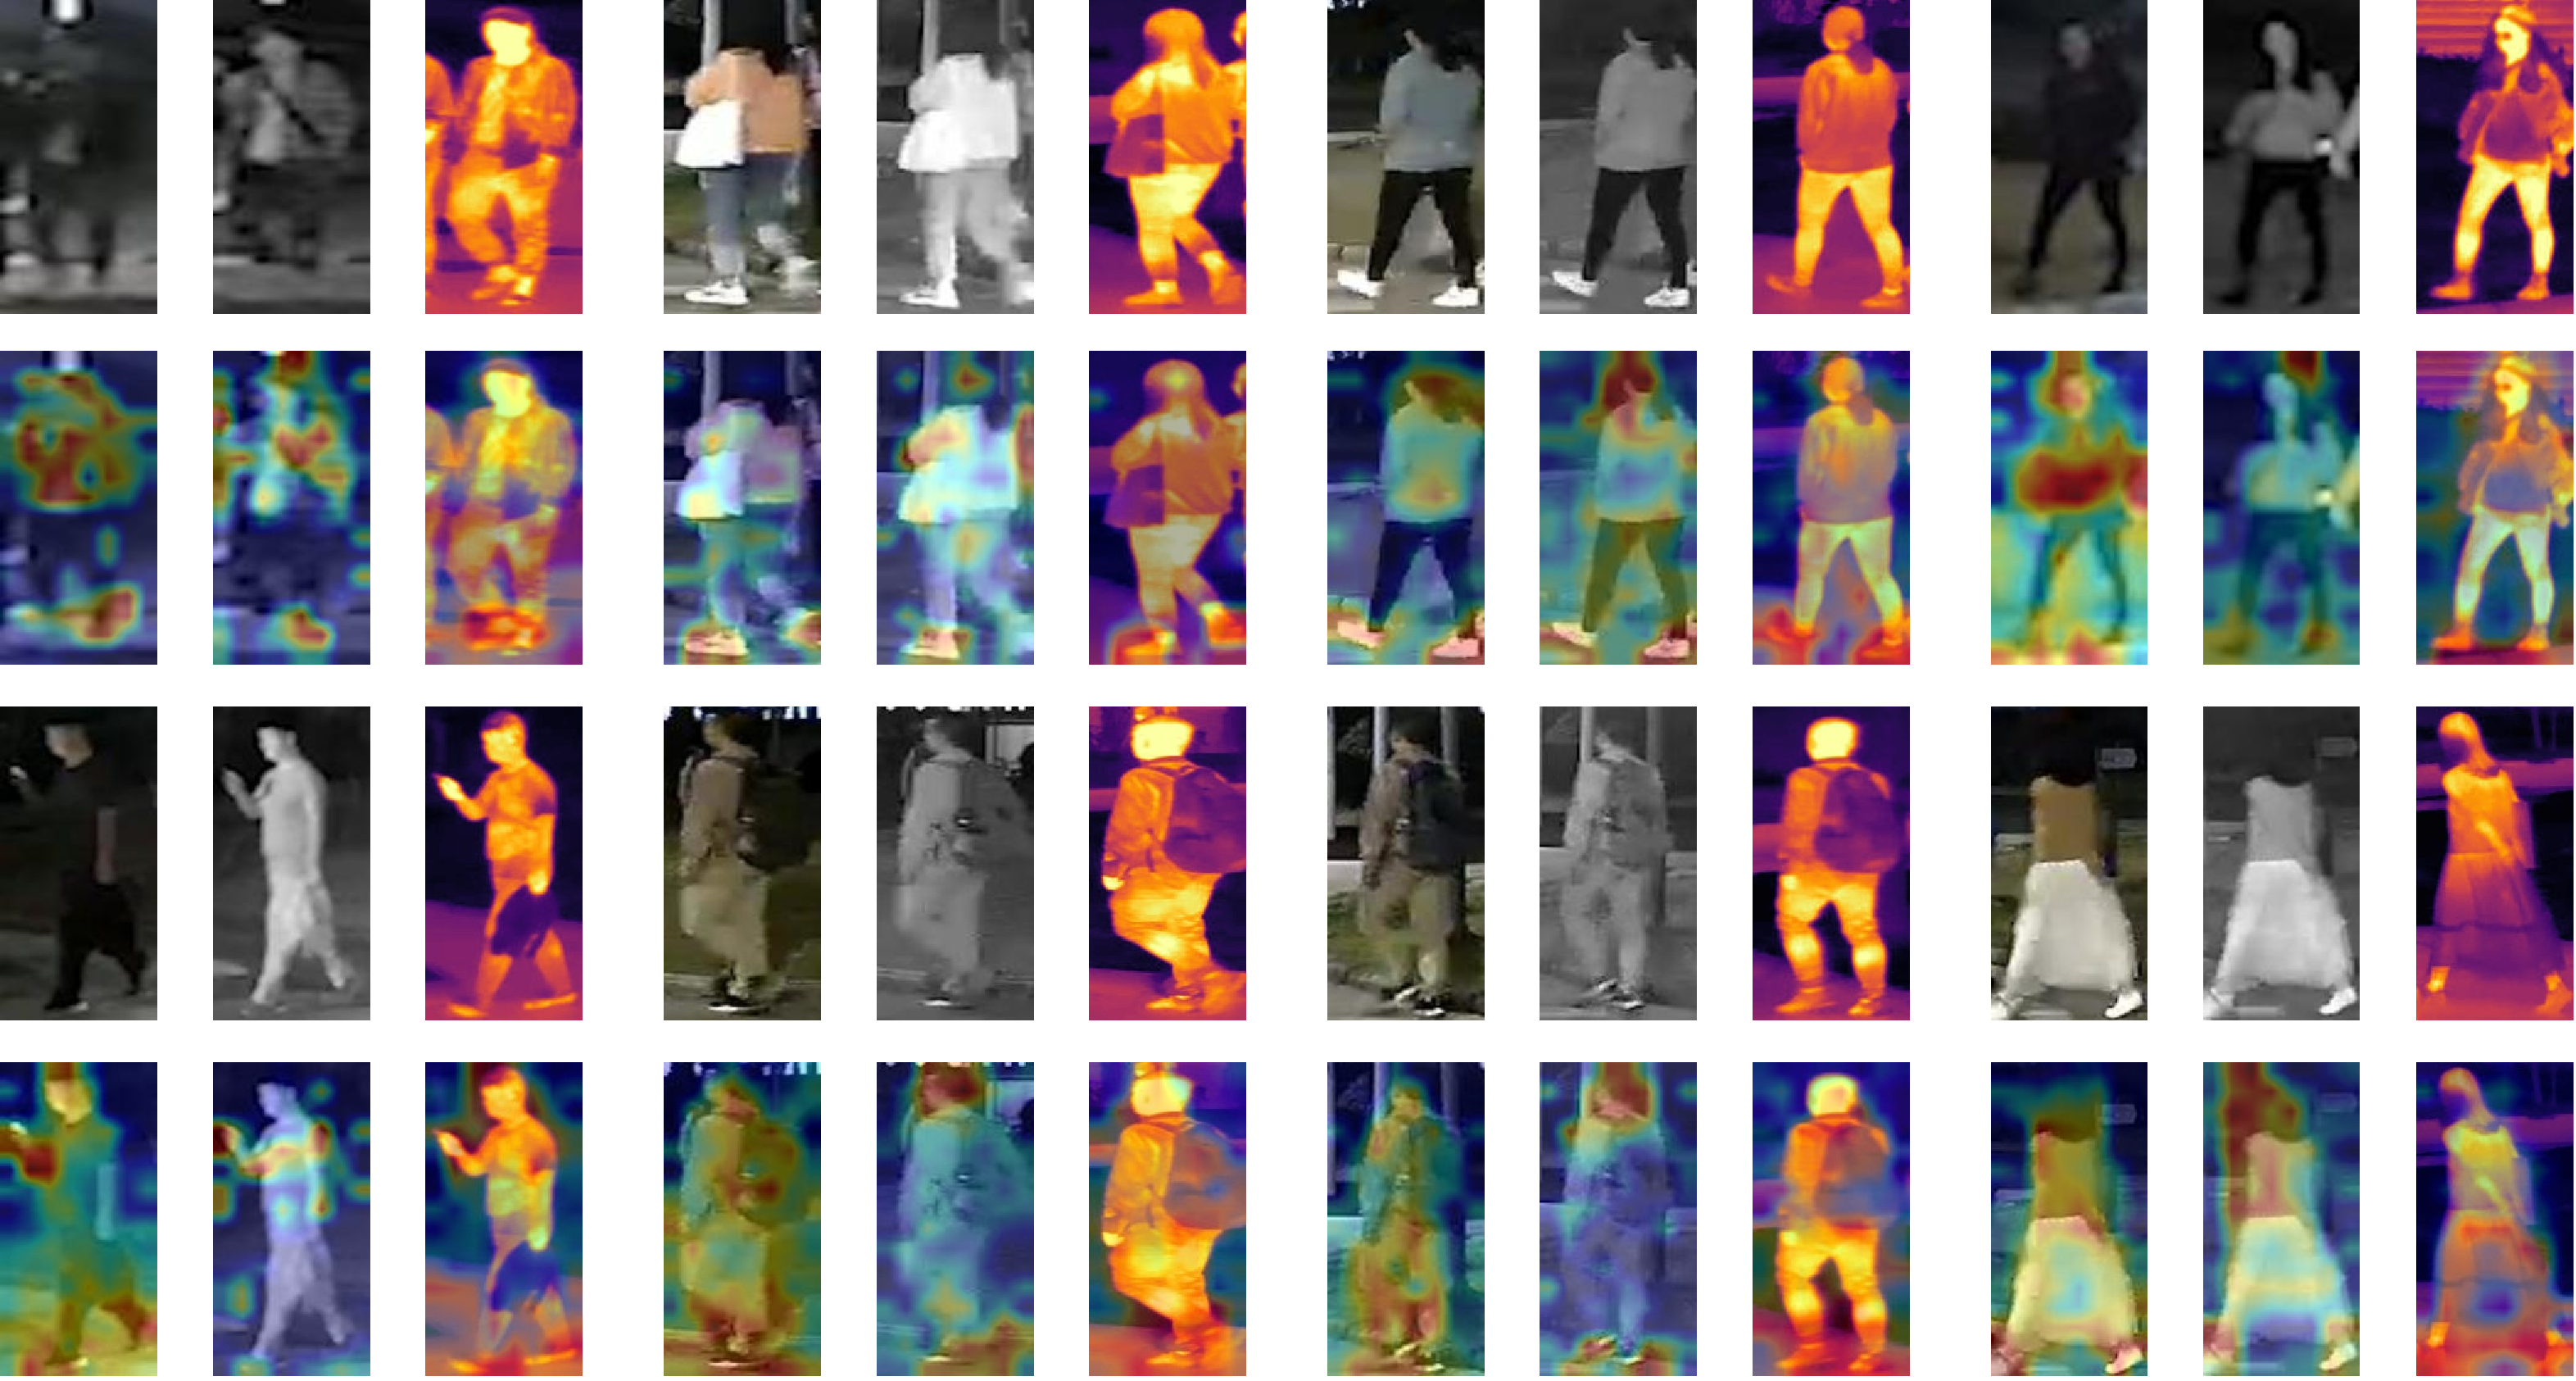
\includegraphics[width=30.\linewidth]{sec/supp_img/SUPP_ACT_MAP.pdf}
  }
  \vspace{-6mm}
   \caption{Visualization of channel activation maps of different modalities on the person ReID dataset.}
  \label{fig:channel_act}
  \vspace{-4mm}
\end{figure}
%~~~~~~~~~~~~~~~~~~~~~~~~~~~~~~~~~~~~~~~~~~~~~~~~~~~~~~~~~~~~~~~~~~~~~~~~~~~~~~~~~~~~~~~~~~~~~~~
\begin{figure}[t]
  \centering
    \resizebox{0.475\textwidth}{!}
    {
  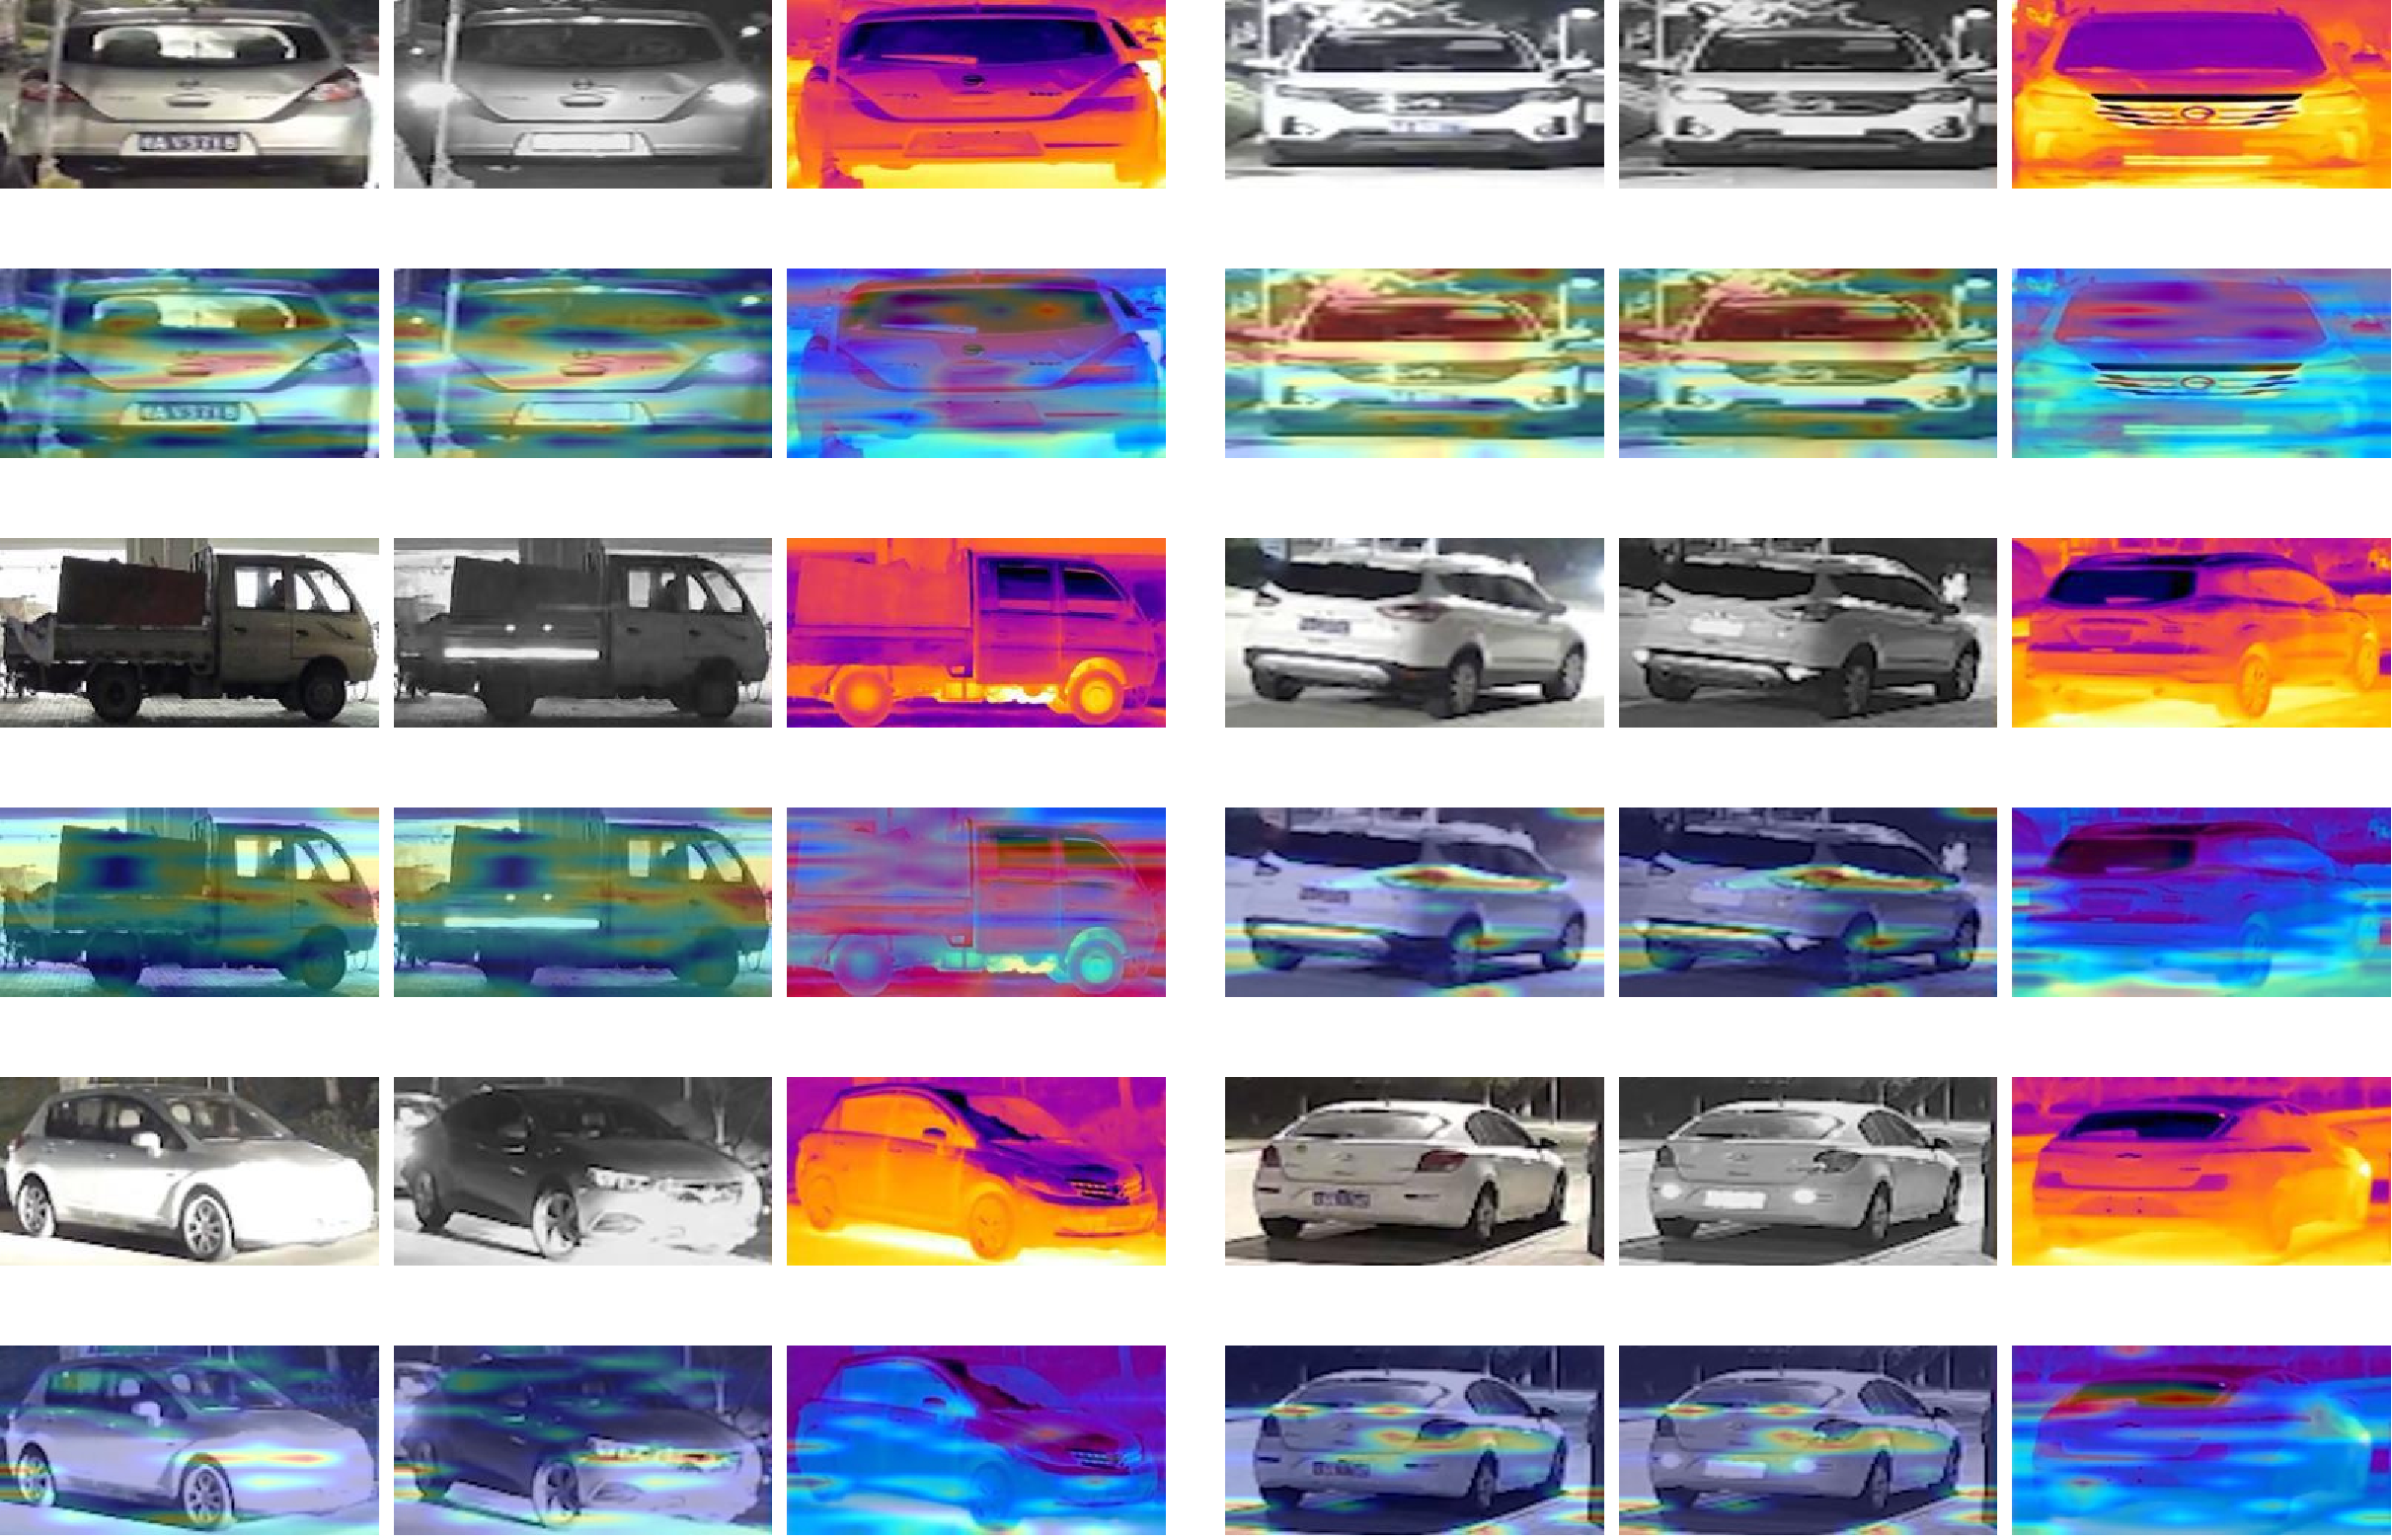
\includegraphics[width=30.\linewidth]{sec/supp_img/SUPP_ACT_MAP_Vehicle.pdf}
  }
  \vspace{-6mm}
   \caption{Visualization of channel activation maps of different modalities on the vehicle ReID dataset.}
  \label{fig:channel_act_vehicle}
  \vspace{-4mm}
\end{figure}
%~~~~~~~~~~~~~~~~~~~~~~~~~~~~~~~~~~~~~~~~~~~~~~~~~~~~~~~~~~~~~~~~~~~~~~~~~~~~~~~~~~~~~~~~~~~~~~~
In \textcolor{red}{Fig.}~\ref{fig:rank_overall}, we present the multi-modal ranking list comparison with different modules on the RGBNT201 dataset.
%
The baseline model without text information exhibits a significant number of incorrect matches, as shown in \textcolor{red}{Fig.}~\ref{fig:rank_overall} (a).
%
By incorporating text information, the model can better distinguish between correct and incorrect matches, as shown in \textcolor{red}{Fig.}~\ref{fig:rank_overall} (b).
%
The introduction of IMFE further enhances the model's ability to identify correct matches, as shown in \textcolor{red}{Fig.}~\ref{fig:rank_overall} (c).
%
Finally, the integration of CDA significantly improves the model's performance, as shown in \textcolor{red}{Fig.}~\ref{fig:rank_overall} (d).
%
These results demonstrate the effectiveness of our proposed modules in enhancing the performance of multi-modal object ReID.
%~~~~~~~~~~~~~~~~~~~~~~~~~~~~~~~~~~~~~~~~~~~~~~~~~~~~~~~~~~~~~~~~~~~~~~~~~~~~~~~~~~~~~~~~~~~~~~~
\\
\textbf{Visualization of Multi-modal Ranking List Comparison with TOP-ReID.}
In \textcolor{red}{Fig.}~\ref{fig:rank_TOP}, we present the multi-modal ranking list comparison with TOP-ReID on the RGBNT201 person dataset.
%
We choose hard examples that TOP-ReID struggles with and compare the performance of our IDEA model.
%
The results verify that our IDEA model consistently outperforms TOP-ReID, achieving accurate matches.
%
\begin{figure*}[t]
  \centering
    \resizebox{0.96\textwidth}{!}
    {
  \includegraphics[width=30.\linewidth]{sec/supp_img/Rank-list-ALL.pdf}
  }
  \vspace{-2mm}
   \caption{Ranking list comparison with different modules on the person ReID dataset RGBNT201.
   %
   (a) Baseline.
   %
   (b) Baseline + Text.
   %
   (c) Baseline + IMFE.
   %
   (d) Baseline + IMFE + CDA.
   %
   The green box indicates the correct match, while the red box indicates the incorrect match.}
  \label{fig:rank_overall}
  \vspace{-2mm}
\end{figure*}
%~~~~~~~~~~~~~~~~~~~~~~~~~~~~~~~~
\begin{figure*}[t]
  \centering
    \resizebox{0.96\textwidth}{!}
    {
  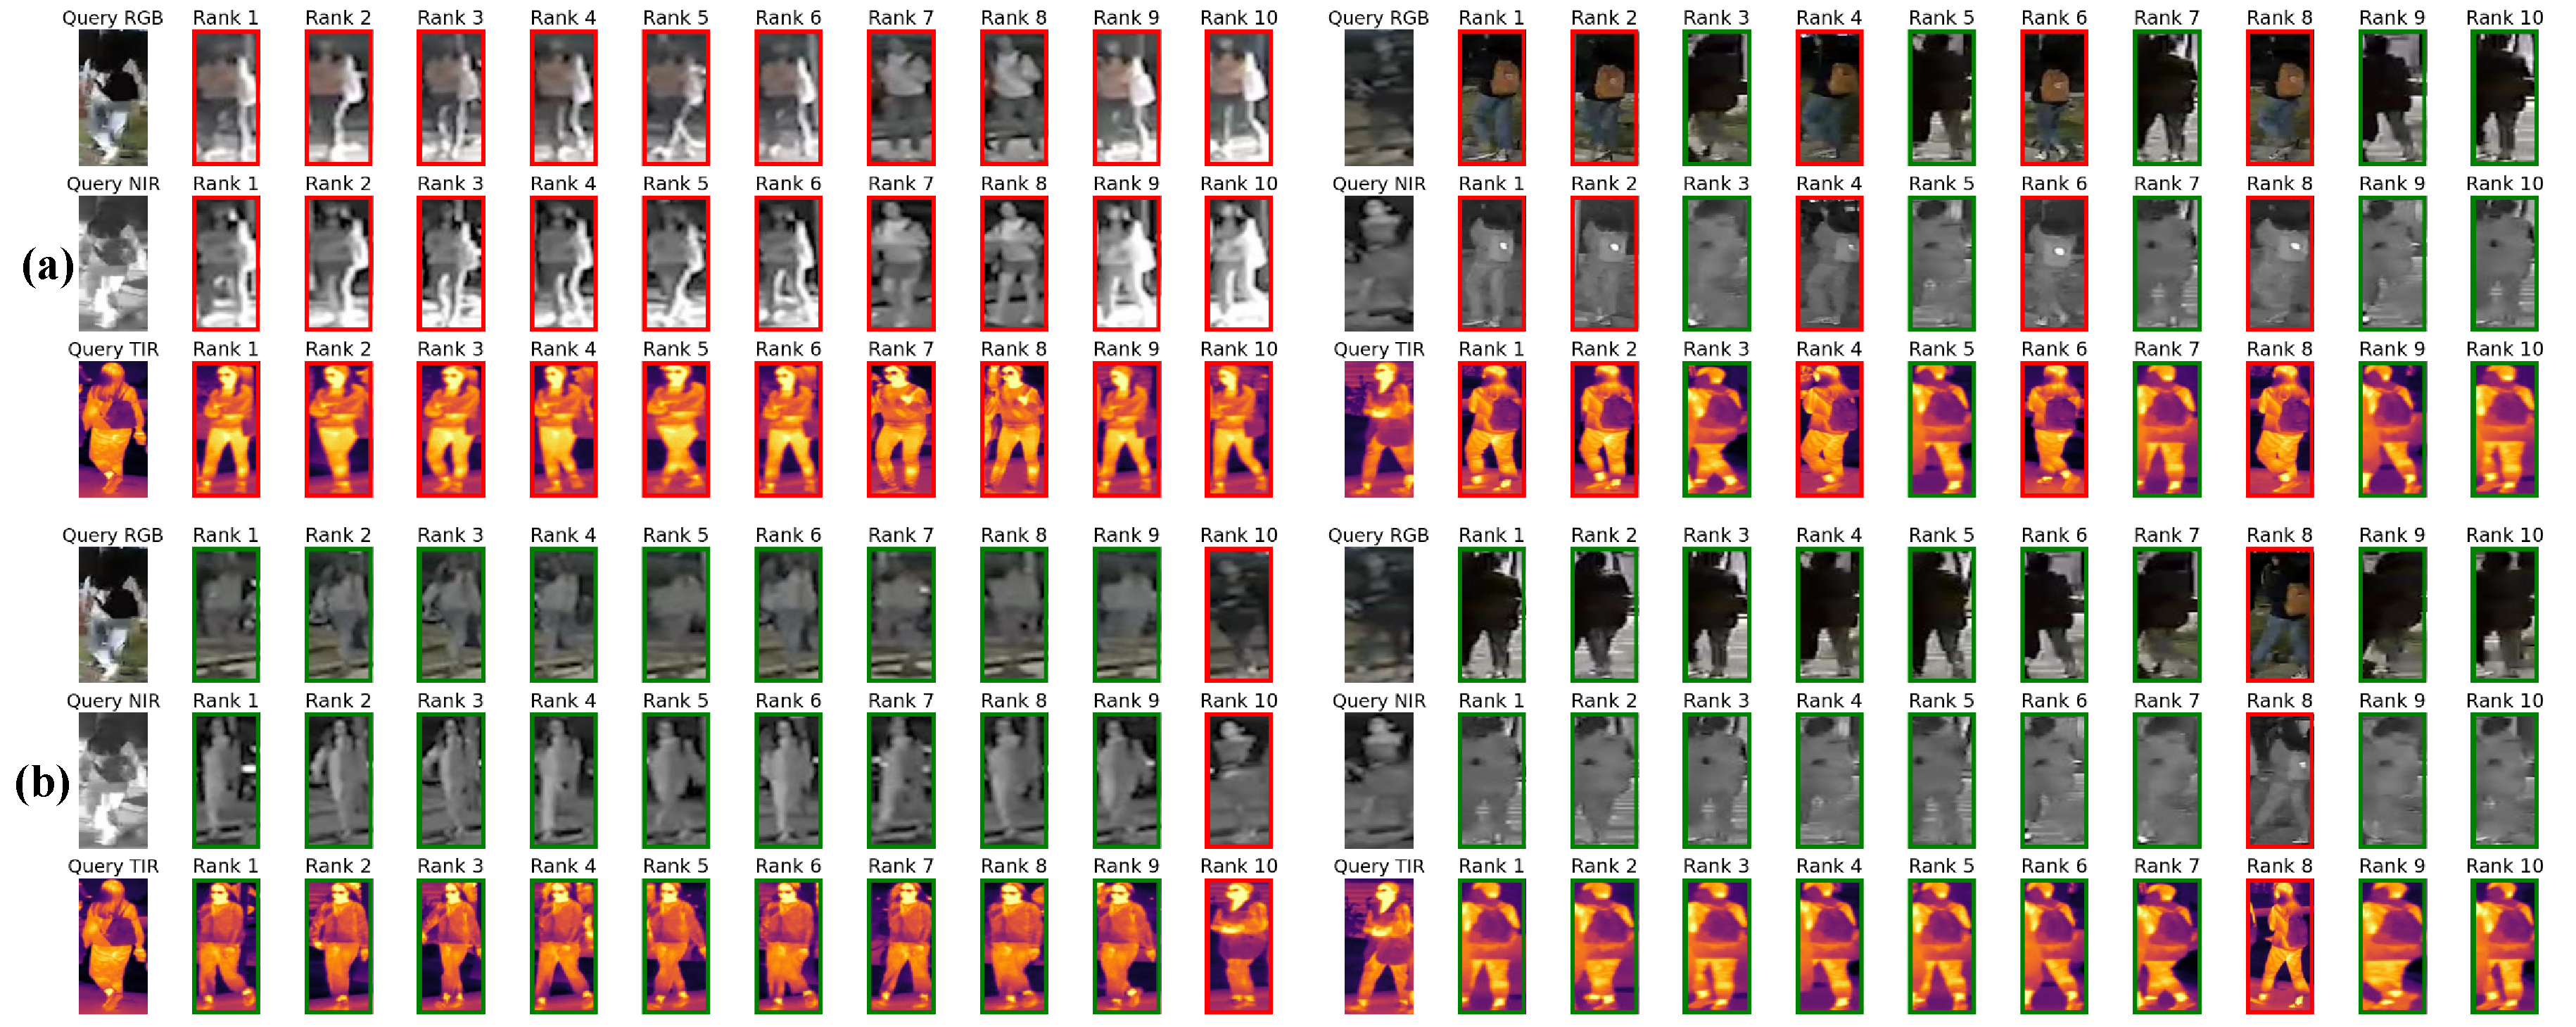
\includegraphics[width=30.\linewidth]{sec/supp_img/Rank-list-TOPReID.pdf}
  }
  \vspace{-2mm}
   \caption{Multi-modal ranking list comparison with TOP-ReID on the person ReID dataset RGBNT201.
   %
   (a) TOP-ReID.
    %
    (b) IDEA.
    %
    The multi-modal ranking list of TOP-ReID is sourced from the supplementary material of DeMo~\cite{wang2024decoupled}.}
  \label{fig:rank_TOP}
  \vspace{-2mm}
\end{figure*}
%~~~~~~~~~~~~~~~~~~~~~~~~~~~~~~~~
\begin{figure*}[t]
  \centering
    \resizebox{0.94\textwidth}{!}
    {
  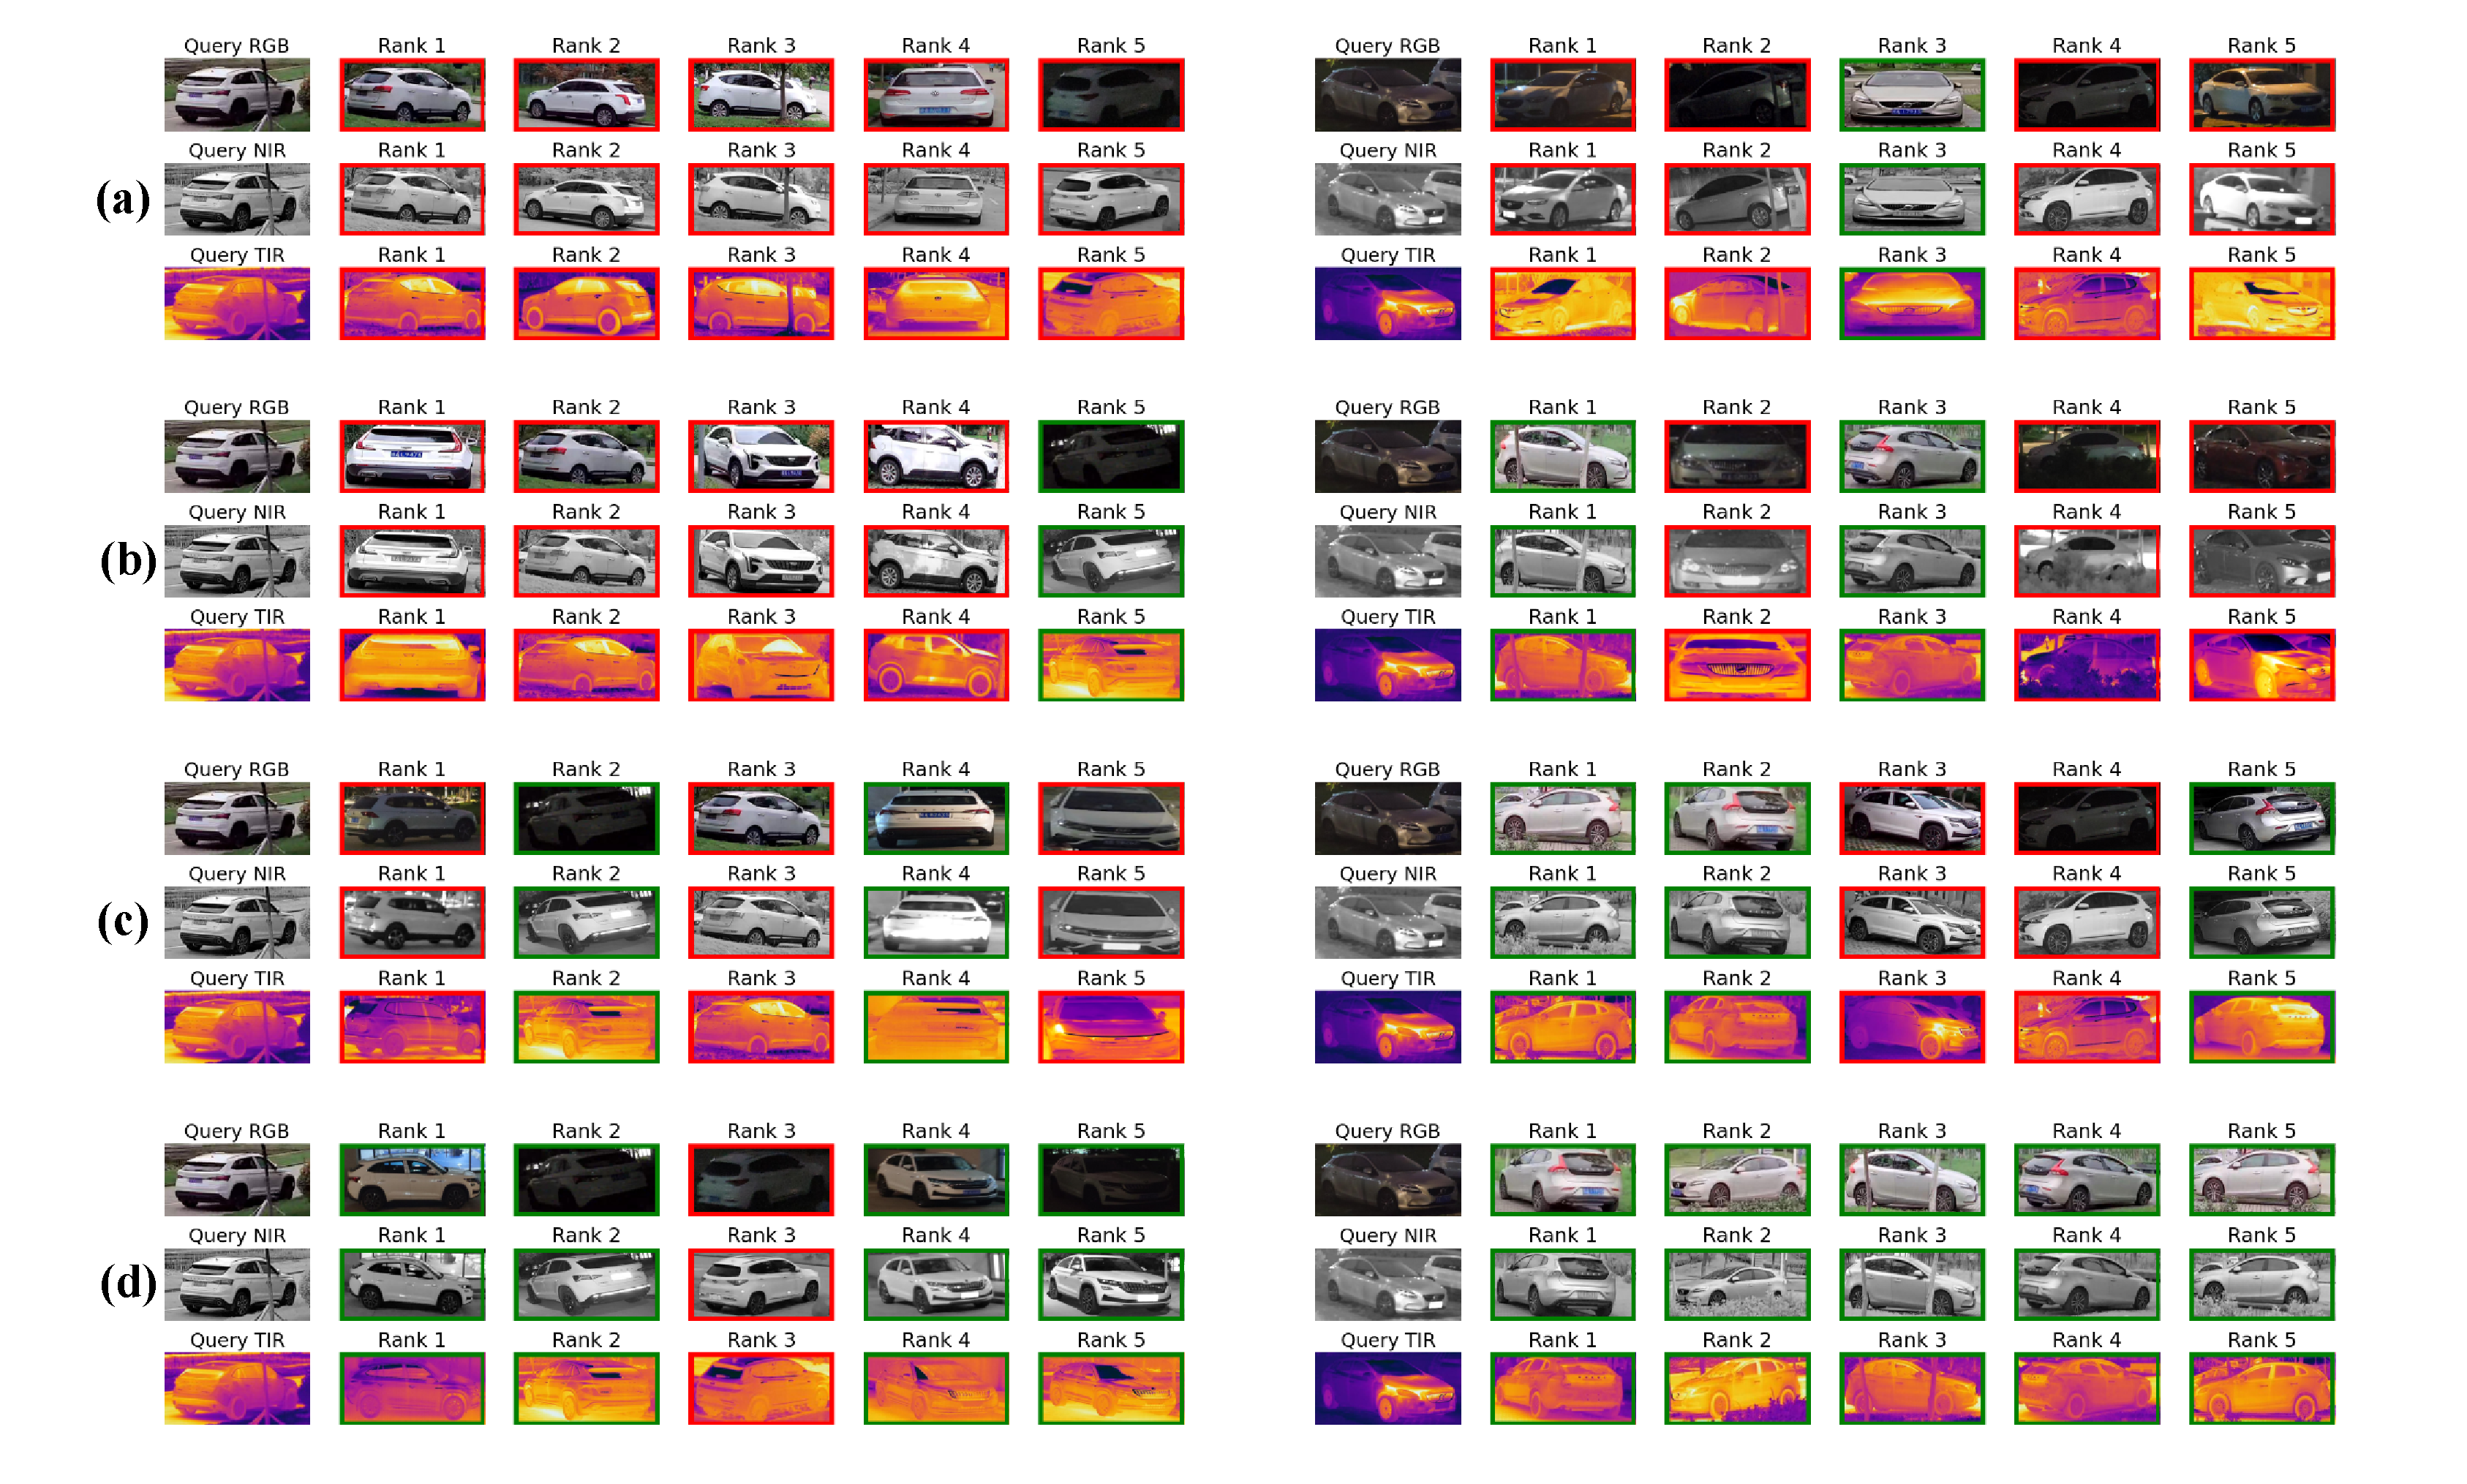
\includegraphics[width=30.\linewidth]{sec/supp_img/Rank_Vehicle.pdf}
  }
  \vspace{-2mm}
   \caption{Ranking list comparison with different modules on the vehicle ReID dataset MSVR310.
   %
   (a) Baseline.
   %
   (b) Baseline + Text.
   %
   (c) Baseline + IMFE.
   %
   (d) Baseline + IMFE + CDA.}
  \label{fig:rank_vehicle_modules}
  \vspace{-2mm}
\end{figure*}
%~~~~~~~~~~~~~~~~~~~~~~~~~~~~~~~~
\begin{figure*}[t]
  \centering
    \resizebox{0.94\textwidth}{!}
    {
  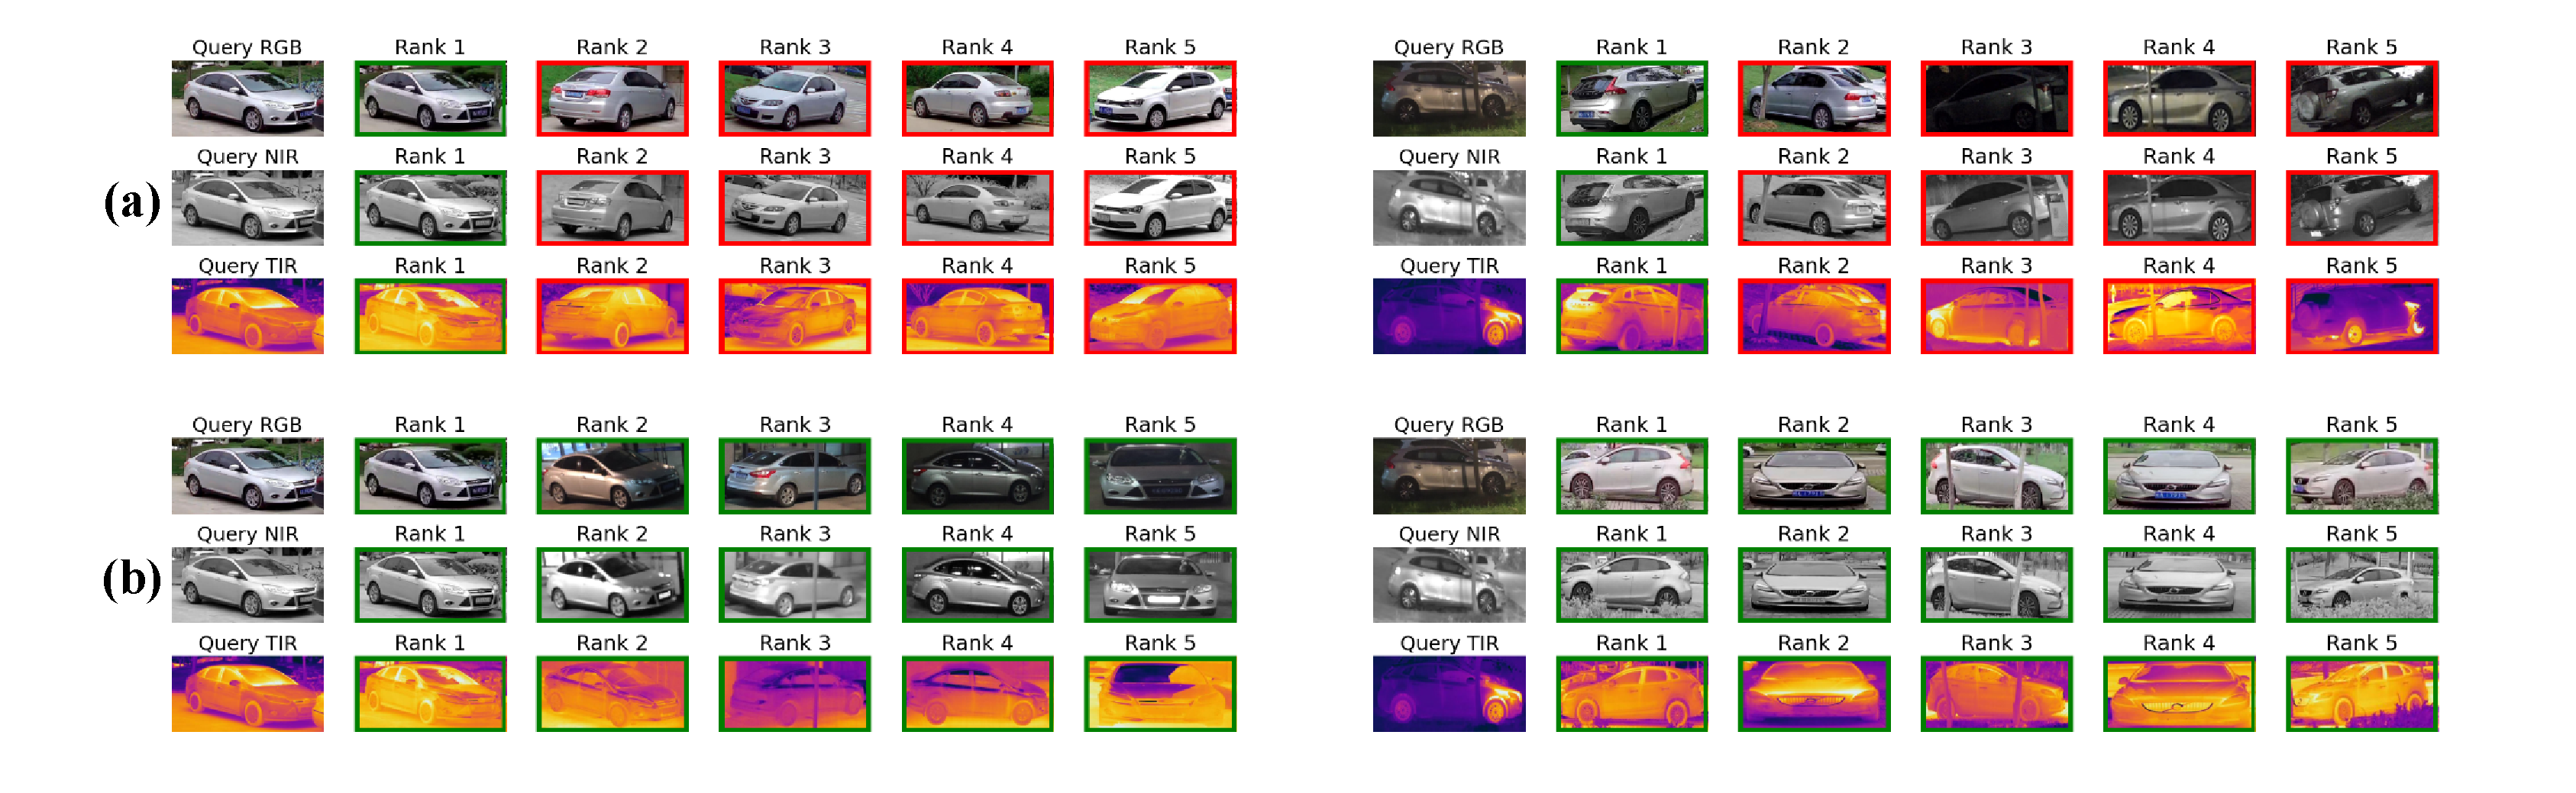
\includegraphics[width=30.\linewidth]{sec/supp_img/Rank_Vehicle_EDITOR.pdf}
  }
  \vspace{-2mm}
   \caption{Multi-modal ranking list comparison with EDITOR on the vehicle ReID dataset MSVR310.
   %
   (a) EDITOR.
    %
    (b) IDEA.}
  \label{fig:rank_EDITOR}
  \vspace{-2mm}
\end{figure*}
%~~~~~~~~~~~~~~~~~~~~~~~~~~~~~~~~
\subsection{More Visualization for Vehicle ReID}
\textbf{Visualization of Channel Activation Maps on the Vehicle ReID Dataset.}
In \textcolor{red}{Fig.}~\ref{fig:channel_act_vehicle}, we present the channel activation maps of different modalities in IDEA on the vehicle ReID dataset.
%
Different modalities focus on distinct semantic regions, such as the corners of the vehicle and the license plate.
%
These activation maps effectively capture discriminative local information, highlighting the importance of leveraging interaction between global features and discriminative local information in multi-modal vehicle ReID.
\\
\textbf{Visualization of Multi-modal Ranking List with Different Modules.}
\textcolor{red}{Fig.}~\ref{fig:rank_vehicle_modules} provides a comparative analysis of multi-modal ranking lists across different module configurations on the MSVR310 vehicle dataset.
%
The baseline model, as seen in \textcolor{red}{Fig.}~\ref{fig:rank_vehicle_modules} (a), relies solely on visual features and fails to reliably distinguish between vehicles with similar appearances, leading to frequent mismatches.
%
Integrating textual information into the model, as shown in \textcolor{red}{Fig.}~\ref{fig:rank_vehicle_modules} (b), greatly enhances the retrieval process, enabling the system to utilize semantic cues for better discrimination.
%
With the introduction of IMFE (\textcolor{red}{Fig.}~\ref{fig:rank_vehicle_modules} (c)), the model demonstrates an ability to capture more nuanced modality-specific information, resulting in a marked improvement in retrieval accuracy.
%
Finally, the addition of CDA (\textcolor{red}{Fig.}~\ref{fig:rank_vehicle_modules} (d)) further refines the ranking results, achieving a level of performance that effectively balances semantic understanding and visual precision.
%
These findings validate the effectiveness of our modules in addressing the challenges of vehicle ReID.
\\
\textbf{Visualization of Multi-modal Ranking List Comparison with EDITOR.}
In \textcolor{red}{Fig.}~\ref{fig:rank_EDITOR}, we compare our IDEA model against EDITOR, the previous state-of-the-art approach on the MSVR310 dataset.
%
EDITOR, while highly effective in many scenarios, struggles with difficult cases involving visually similar vehicles or missing modality-specific details.
%
This limitation is evident in its inability to consistently rank correct matches, especially when semantic guidance is needed to resolve ambiguities.
%
In contrast, our IDEA model leverages advanced multi-modal modules to seamlessly integrate visual and textual cues, resulting in a dramatic reduction in errors even for the hard cases.
%
This comparative analysis highlights IDEA's superiority over EDITOR, verifying its robustness in tackling real-world challenges.
